\documentclass[journal]{IEEEtran}
\usepackage[T1]{fontenc}
\usepackage{amsmath,amssymb}
\usepackage{graphicx}
\renewcommand{\thefigure}{S\arabic{figure}}
\usepackage{booktabs}
\usepackage{algorithm}
\usepackage[noend]{algpseudocode}
\usepackage{url}
\usepackage[hidelinks]{hyperref}
\usepackage{microtype}
\renewcommand{\thetable}{S\arabic{table}}
\renewcommand{\thealgorithm}{S\arabic{algorithm}}
\algrenewcommand\algorithmiccomment[1]{\hfill$\triangleright$ #1}
\makeatletter
\renewcommand{\@IEEEsectpunct}{.\ \,}
\makeatother


\begin{document}
\title{Supplementary Material for ``Paths, Completion, or Both? A t-Norm Audit and a Pre-Specified Test of Hedging Across Missingness Patterns in a Graded Health Knowledge Graph of Depressive Symptoms''}
\author{Truong~Hai~Bang$^{a,*}$ and~Van~An~Phan~Thi$^{b}$%
\thanks{$^{a}$Faculty of Engineering and Computer Science, Saigon International University, 8C Tong Huu Dinh Street, An Khanh Ward, Ho Chi Minh City, Vietnam. $^{b}$VNU University of Education, Vietnam National University, Hanoi, G7 Building, No.~144 Xuan Thuy Street, Cau Giay District, Hanoi, Vietnam (e-mail: phanthivanantlls@gmail.com). $^{*}$Corresponding author: Truong Hai Bang (e-mail: truonghaibang@siu.edu.vn; telephone: +84~918~264~026).}}
\markboth{IEEE Journal of Biomedical and Health Informatics, Supplementary Material}{}
\maketitle

\section*{Supplementary Methods}

\emph{Implementation.} Python 3.13 with NumPy 2.5, pandas 3.0, scikit-learn 1.9 and SciPy 1.18; master seed 20261029. A released check script confirms that $S_0$ equals the weighted mean of $j$ for crisp $i$. \texttt{fast\_compose.py} (Algorithm~S2) reproduces the enumeration of \texttt{rq3x.paths} exactly on the NHANES relation. The graph construction, the leave-dyad-out test, the binarization test and the clinical review form, with the reviewer's entries, are documented in the repository (\texttt{graph2.py}, \texttt{rq3x.py}, \texttt{analysis2.py}, \texttt{review/}). Checks are released by version: \texttt{rigor\_checks.py} (v1.8.0, commit \texttt{ca60d43}), \texttt{scale\_checks.py} (v1.9.0, commit \texttt{4908dba}) and \texttt{replicate\_checks.py} with \texttt{figures9.py} (v1.10.0), \texttt{pcc\_experiments.py} (v2.0.0), \texttt{pcc\_checks.py} with \texttt{nhanes\_l.py} (v2.1.0), \texttt{pcc\_limits.py} (v2.2.0) and \texttt{report\_checks.py} (v2.3.0, extended in v2.3.1, v2.3.2 and v2.3.3), which recomputes regrets, worst-case designs and rounding from the stored results without refitting.

\emph{Masking, tuning and nested validation.} Table~S7 lists, for each design, the outer withheld set, how tuning parameters are chosen and which quantities are recomputed after masking. Two rules hold in every design: both directions of a withheld dyad are removed together, in the outer mask and in every inner cross-validation fold; and the target relation is never used for any choice. In the single-dyad design of main Table~I the completion rank, the soft-impute penalty and the embedding settings were chosen once by five-fold dyad cross-validation on the full development matrix, so the withheld dyad was among the cells used for that choice, though never for fitting. The nested check removes the outer dyad first and then runs the five-fold inner cross-validation on the remaining 275 dyads (seed $i\cdot24+j$ for dyad $(i,j)$). Ranks chosen: 3 in 243 masks, 4 in 31, 5 in 2; penalties chosen: 0.6 in 241, 0.3 in 34, 0.1 in 1. Because 0.6 is the largest value of the grid $\{0.01,0.03,0.1,0.3,0.6\}$, we repeated the choice on a grid extended to 1, 2 and 5. Cross-validated $\rho$ by penalty was 0.786, 0.861, 0.906, 0.913, 0.917, 0.920, 0.916 and 0.886; chosen once, $\lambda=1$ gave held-out $\rho=0.917$ (0.918 at $\lambda=0.6$). Inside the 276 masks the extended grid chose 1 in 201, 0.6 in 66 and 2 in 9, never 5, with $\rho=0.916$. In the block design the extended grid gave a pair-weighted mean of 0.651 (0.639 on the original grid). The soft-impute scale is chosen with the penalty: in the single-dyad design by dyad cross-validation on the development matrix (logit 0.917, raw 0.888), and in the block design by cross-validation on the other blocks, which chose the logit scale in all 10 blocks. Katz uses damping $0.5/\lambda_{\max}$, with $\lambda_{\max}$ the spectral radius of the input matrix (in the single-dyad design, the development matrix before masking); personalized PageRank restarts with probability 0.15. The logit transform is $\operatorname{logit}\{(\mu+0.005)/(1-\mu+0.005)\}$, with a fixed offset, the same in every design. The Adamic--Adar and resource-allocation weights use the strength of the intermediate $k$, which does not include the withheld edges.

\emph{Direction: exact decomposition and its approximation (Table~S5).} For a dyad with both directions positive, $\mu_{ij}=s_{ij}\sqrt{r_{ij}}$ holds exactly with $r_{ij}=\mu_{ij}/\mu_{ji}$; main Eq.~(4) shows that cancellation along paths needs $\varepsilon_{ikj}=r_{ik}r_{kj}/r_{ij}=1$. For crisp concepts on common respondents $r_{ij}=o_j/o_i$ (main Proposition~1), so $\varepsilon=1$. Table~S5 reports, on the development relation, how far the graded relation departs from this: the path-cancellation error over triples in which all three dyads are positive, the error of replacing $r_{ij}$ by the odds ratio $R_{ij}$ of survey-weighted mean activations, and the agreement of directed and re-directed product composition. Across the 221 pairs with both directions above 0.01, $\log(\mu(i\to j)/\mu(j\to i))$ tracked $\operatorname{logit}p_j-\operatorname{logit}p_i$ with $r=0.997$ (slope 1.05): $r=0.9999$ over the six unordered crisp--crisp dyads with both directions at or above 0.01, which are every pair among hypertension, cardiovascular disease, cancer and arthritis (uninsured, the fifth crisp concept, has no positive relation with any of them), 0.998 (residual SD 0.088) for the 143 pairs involving a PHQ-9 item and 0.993 (residual SD 0.127) for the other 72 graded pairs. The crisp--crisp correlation is not exactly 1 because each pair uses its own respondents while $R$ uses full-sample prevalences. On the raw subsethood, 11 of 24 concepts had their strongest relation to poor self-rated health and 8 to obesity, the two most prevalent concepts; after correction the strongest targets spread across fatigue (6), hypertension (5), low income (4) and others. Clipping: 49 ordered pairs (25 dyads) had negative excess in development and 48 (24 dyads) held out; 503 and 504 ordered pairs were positive, and 468 and 474 reached 0.01.

\emph{Composing the symmetric relation and re-directing it.} With $s_{ij}=\sqrt{\mu(i\to j)\mu(j\to i)}$ composed by each t-norm and multiplied by $\sqrt{o_j/o_i}$ from development prevalences, $\rho$ over the 552 directed pairs was 0.879 for the product (directed composition 0.878), 0.822 for Hamacher (0.854), 0.756 for the minimum (0.730), 0.484 for Yager and 0.086 for {\L}ukasiewicz; rank-3 completion of $s_{ij}$ re-directed reached 0.908 (0.908). The direction factor alone reached 0.520. JRR intervals: product $-$ Hamacher after re-direction 0.056 [0.044, 0.069]; rank-3 $-$ product 0.029 [0.005, 0.053]. In the 20 split halves the re-directed product was first in all 20.

\emph{Recalibration before re-direction (Table~S17).} Re-direction multiplies the composed symmetric value by $\sqrt{o_j/o_i}$, so the result ranks well only if the composed value is on the multiplicative scale of $s$. For each t-norm we mapped the composed symmetric relation $C$ onto the scale of $s$ before re-direction in two ways, each leave-dyad-out over the 276 dyads: a power map $C\mapsto cC^a$, fitted by least squares of $\log s$ on $\log C$ over the other dyads with $s\ge0.01$ and $C>0$; and isotonic regression of $s$ on $C$ over all other dyads. The constant $c$ does not affect ranks. JRR intervals re-fit both maps in every replicate. For Yager and {\L}ukasiewicz most composed values are 0, so the power map is undefined and only the isotonic map is reported.

\emph{Cold start with one anchor.} With $m=1$ the median per-concept $\rho$ of soft-impute on the logit scale was 0.389 with the penalty chosen on the observed relations (0.6 in 100 of 120 concept-repetitions, 0.3 in the rest), 0.390 with the extended grid, 0.409 at $\lambda=5$ and 0.401 on the raw scale; rank-3 completion reached 0.600 in the same five repetitions. On the logit scale the predictions for the withheld row had a median standard deviation of 0.20 times that of the observed relations, so the nuclear-norm penalty shrinks the almost empty row toward the overall mean. Splitting concepts at the median strength of their single anchor, soft-impute reached 0.28 with a weak anchor and 0.47 with a strong one; rank-3 completion 0.55 and 0.64.

\emph{Block-wise rank-1 completion.} Within each of the 16 ordered relation-type blocks, a rank-1 matrix was fitted by iterated SVD to the block's other cells (both directions of the dyad and the diagonal masked) and used to predict the withheld cell.

\emph{Replicate distribution in the block design (Fig.~S1).} In Table~S8 the rank of rank-3 completion is fixed at 3 in the full sample and in every JRR replicate; soft-impute and ComplEx settings are re-chosen. The 90 replicate values of product $-$ rank-3 completion (pair-weighted mean of within-block $\rho$; full sample 0.291) ranged from 0.137 to 0.302 and were all positive; 88 lay between 0.279 and 0.302. The two others, 0.137 each, are development replicates in which rank-3 completion of the lifestyle--health block reached $\rho$ 0.76 (0.755) and 0.73 (0.727) instead of $-0.65$; this block contributes 98\% of the JRR sum of squares, and the other blocks at most 1\% each. The distribution is therefore a tight cluster with two outliers, not two modes, and the normal-approximation interval $[-0.141, 0.723]$ overstates the uncertainty; it is reported as descriptive. With the rank re-chosen on the other blocks by five-fold dyad cross-validation in the full sample (ranks 3, 2, 4, 3, 5, 3, 2, 5, 3, 3 for the ten blocks) and in every replicate (rank 2 in 193, 3 in 409, 4 in 120 and 5 in 178 of the 900 block fits), product $-$ rank-$k$ was 0.220 ($-0.315$ to 0.755); the replicate values ranged from 0.132 to 0.287, all positive, in two clusters near 0.22 and 0.27 according to the ranks chosen, with 73\% of the sum of squares from the symptom--health block and 25\% from lifestyle--health. For comparison, the replicate values of product $-$ Katz ranged from $-0.004$ to 0.005 and those of product $-$ Hamacher from 0.068 to 0.079. Script: \texttt{replicate\_checks.py blockreps}.

\emph{Shrinkage.} The Kish effective sample of a pair uses the weights $w_n\min(a_{n,i},a_{n,j})$ over respondents observed on both concepts (median 657 over the 552 ordered pairs; 24 pairs below 100). Each relation was shrunk towards the mean of the other pairs of its ordered type block with weight $n_{\mathrm{eff}}/(n_{\mathrm{eff}}+\kappa)$, $\kappa\in\{50,100,300\}$ ($\kappa=100$: product 0.858, Hamacher 0.842, rank-3 0.881).

\emph{Jackknife repeated replication and coverage.} Each period pools three two-year cycles with 15 strata each, treated as 45 distinct strata. In each stratum the PSU with the lower NHANES code (\texttt{SDMVPSU}~$=1$) is deleted and the weights of the other are doubled. Each replicate rebuilds the relation of its period with the other period kept at full sample, re-chooses ranks and penalties, and recomputes every predictor on the same masks, so differences are paired. $SE^2=\sum_r(\hat\theta_r-\hat\theta)^2$ over the 90 replicates of the cross-period design (60 in the pre-specified test), which adds the variances of the two independent periods, and intervals are $\hat\theta\pm1.96\,SE$. The split-half design draws half of the PSUs of each stratum and rescales both halves to the full weight total. Randomness from masks, anchors and embedding initialization is not in the JRR; random-mask designs report the standard deviation over repetitions, with the same mask for every predictor within a repetition. Coverage was checked in a clustered respondent-level simulation (Table~S10): a three-factor latent model with PHQ-like ordinal and binary measurement, 45 strata $\times$ 2 PSUs $\times$ 170 respondents per sample, PSU random effects on the factors (intraclass correlation 0.05), two independent samples per replicate, truth from two samples nine times as large, JRR with 90 replicates; 100 simulation replicates. The completion rank was fixed at 3 in this simulation, whereas the intervals in main Table~I re-choose it in every replicate (rank 3 in 90 of 90 replicates), so the simulation calibrates the intervals of the fixed procedure only. An earlier run of 24 replicates also computed bias-shifted Rao--Wu percentile intervals from 20 bootstrap replicates.

\emph{Equivalence tests (Table~S24).} For a difference $d$ with JRR standard error $SE$, the two one-sided tests reject $|d|\ge\delta$ when the 90\% interval $d\pm1.645\,SE$ lies inside $(-\delta,\delta)$; the $p$-value is $\max\{\Phi(-(d+\delta)/SE),\Phi(-(\delta-d)/SE)\}$. For the pre-specified cycle $SE$ is recovered from the reported 95\% interval. The margins $\delta=0.03$ and $0.05$ were set after the pre-specified test was run. The margin 0.03 is of the order of the change in one method's $\rho$ when only the target sample changes: across the cross-period, split-half and swapped designs of main Table~I a method's $\rho$ moved by 0.009 (product) to 0.023 (Hamacher), and on symmetric relations (Table~S11) by up to 0.037.

\emph{Respondent-level chained versus factor simulation.} The chained model is a sparse random directed acyclic graph (edge probability 0.12, coefficients 0.3--0.7) along a random order, with each variable the weighted sum of its parents plus Gaussian noise; factor models have one or three factors with loadings 0.4--0.8 plus 0--0.25 cross-loadings and noise SD 0.8. Continuous scores were cut into the data's scales (ordinal 0--3 at the 70th, 88th and 96th percentiles for the nine items; binary at the 75th percentile otherwise), 15,000 respondents per sample, 60 replicates per model. Product best t-norm: chain 60/60, one factor 25/60, three factors 22/60; rank-3 above product: 57\%, 8\% and 100\%. A second run (30 replicates per model) added continuous measurement, $a=\Phi(z-c)$ with $c=0.9$ for items and 0.7 otherwise, and the block design. Product best t-norm with cut and continuous scales: chain 100\% and 100\%, one factor 40\% and 97\%, three factors 47\% and 43\%. The partial correlation of the product's predictions given completion's was 0.78 under one factor, against 0.30 observed, which rules out a single factor; it was 0.28 under chaining and 0.20 under three factors, which it cannot separate. With whole types withheld, pair-weighted $\rho$ (product, rank-3, soft-impute, Katz), cut scales: chain 0.566, 0.550, 0.537, 0.578; one factor 0.958, 0.530, 0.917, 0.970; three factors 0.895, 0.977, 0.936, 0.761; continuous: 0.576, 0.558, 0.556, 0.590; 0.978, 0.480, 0.978, 0.982; 0.905, 0.988, 0.977, 0.780. The product beat rank-3 completion in 63\% of chained, 100\% of one-factor and 0\% of three-factor replicates, and Katz beat the product in most chained and one-factor replicates, so the block result in the data does not identify chaining either.

\emph{First public release and pre-specified test.} The first public release of the code (tag v1.0.0, 30 October 2026; Zenodo 10.5281/zenodo.23790457) compared the five t-norms with a strength-product and a block-mean baseline; completion, link-prediction indices and embeddings were added later. The pre-specified plan (\texttt{confirmatory/PLAN.md}) was added by commit \texttt{0ba672c} at 06:49:47 UTC on 16 November 2026. The commit that adds cycle D to \texttt{download\_nhanes.py}, the checksums of the 2005--2006 files in \texttt{raw/MANIFEST.md5}, \texttt{confirmatory/run\_2005.py} and the 2005--2006 results is \texttt{a372f21}, at 08:16:32 UTC on the same day. No separate time stamp of the download exists, and git commit times are set by the committer; the order therefore rests on the repository history. The 2005--2006 cycle has 15 strata; the JRR used $45+15$ replicates. Results are in Table~S30. The post-pre-specification equivalence tests (Table~S24) were added in v1.8.0 (commit \texttt{ca60d43}, 08:54:59 UTC). The plan contained no power calculation and did not name the soft-impute scale for H4; \texttt{run\_2005.py} used the raw scale. Table~S14 gives, for each rule, the probability that it is met when the true difference is 0, 0.03 or 0.05, from the 2005--2006 JRR standard errors (normal approximation: $\Phi(\Delta/SE-1.96)$ for a directional rule; $\Phi(1.96-\Delta/SE)-\Phi(-1.96-\Delta/SE)$ for a rule met when the 95\% interval contains 0). With the logit scale, chosen by cross-validation on the other blocks in all 10 blocks, product $-$ soft-impute in the pre-specified block design was 0.086 [$-0.002$, 0.174] (raw scale, as pre-specified: 0.143 [0.073, 0.213]); this secondary analysis was added in v1.9.0 and is exploratory.

\emph{Pre-specified test on NHANES 2021--2023 (Table~S29).} The plan (\texttt{confirmatory/PLAN\_2021.md}) and the code that maps cycle L (\texttt{nhanes\_l.py}) were committed in \texttt{372dfee}; GitHub's repository activity log records the push of that commit, which created the branch carrying it, at 06:13:17 UTC on 22 November 2026, and the 13 cycle-L files were then fetched by \texttt{download\_nhanes.py L} (our own log: 06:13:20--06:13:32 UTC); their checksums are appended to \texttt{raw/MANIFEST.md5} in the commit that adds the results. Before the plan only the public codebooks were read. Mapping: marital status from \texttt{DMDMARTZ} (married or living with partner 0, widowed/divorced/separated 1, never married 0.5); self-rated health from \texttt{HUQ010}, because \texttt{HSQ\_L} holds no general-health item; inactivity 0 if any vigorous leisure-time activity (\texttt{PAD810Q} $>0$), 0.5 if only moderate (\texttt{PAD790Q} $>0$), 1 otherwise, with codes 7777 and 9999 missing. Every other concept used the \texttt{clean2.py} definitions without change. The PHQ-9 was self-administered by audio computer-assisted interview in this cycle. One change was made to the analysis code after the plan was committed and before any cycle-L result was computed: the raw-scale blend used in the JRR part was set to $\lambda=0.03$, the value used when its weight was chosen, instead of PCC's $\lambda$; the primary hypotheses do not involve it. No deviation from the plan occurred in the primary and secondary analyses.

\emph{Illustrative query in split halves.} Each of the 20 PSU halves of 2013--2018 predicted the other half and the 2007--2012 relation; each candidate relation was predicted with only its own dyad withheld. Mean (range) number of symptoms whose top modifiable correlate was recovered, half to half: product 7.9 (7--9), rank-3 completion 8.35 (7--9), direct edge 7.75 (7--8), Hamacher 6.5 (4--8), minimum 2.65 (0--5.5; tied top prediction in 2.95 symptoms on average); half to 2007--2012: 7.45, 7.0, 7.6, 6.25 and 3.0. The product scored above the minimum in all 20 halves in both designs. Per-symptom answers are in Table~S9. Development gap between the first and second of the five modifiable correlates for $\mu(c\to s)$: anhedonia 0.043 (smoking over short sleep), depressed mood 0.056 (same), sleep problems 0.001 (short sleep over smoking), fatigue 0.018 (smoking over short sleep), appetite change 0.038 (smoking over heavy drinking), worthlessness 0.039 (same), poor concentration 0.046 (smoking over short sleep), psychomotor change 0.027 (same), thoughts of self-harm 0.011 (smoking over inactivity). The two halves of a split hold complementary PSUs of every stratum, so their deviations from the full sample in the leader's margin mirror each other (correlation $-1.00$ over the 20 splits for every symptom). When the full-sample margin is small, the leader of one half therefore tends to trail in the other: the halves agreed on the leader in 0 of 20 splits for sleep problems and 15 of 20 for fatigue, and in all 20 for the other seven symptoms. This is why the direct edge recovers fewer answers than the product in this design and is a ceiling only for the cross-period design. Script: \texttt{replicate\_checks.py querygap}.

\emph{Further measures.} The hop count of the shortest indirect path in thresholded copies serves as a binary baseline ($\rho$ 0.591 at the median, 0.556 at $\mu\ge0.25$). On non-zero predictions Yager reached $\rho=0.766$ (146 pairs) and {\L}ukasiewicz 0.672 (23 pairs). Per-source ranking: NDCG@5 0.872 for the product, 0.903 for rank-3 completion and 0.917 for cross-validated soft-impute.

\emph{Run time (Table~S22).} Wall-clock times of a single Python process on the machine used for the analyses; the 90-replicate totals are the time of one replicate multiplied by 90. PCC times are per fit or per iteration; for $n=400$ the best-path step holds an $n^3$ array (0.5 GB in double precision), so larger graphs need the best intermediates computed block by block and a truncated or randomized SVD.

\emph{Exact composition in cubic time (Algorithm~S2).} Maximizing over $k$ in $T(a_{ik},a_{kj})$ is a matrix product over the $(\max,T)$ semiring and costs $O(n^3)$, as in the Floyd--Warshall recursion \cite{floyd1962}; the leave-dyad-out constraint is what prevents reusing one product for three edges, and enumeration costs $O(n^4)$. Two properties shared by all t-norms remove the fourth power: $T$ is nondecreasing in each argument, so $\max_kT(x_k,y)=T(\max_kx_k,y)$ for any finite set, and $T(0,x)\le T(0,1)=0$.

\emph{Proposition.} For any t-norm $T$ and a relation with zero diagonal, Algorithm~S2 returns $\hat\mu_T(i\to j)$ of main Eq.~(5) for every ordered pair in $O(n^3)$ time. \emph{Proof.} For two edges, terms with $k\in\{i,j\}$ vanish because $a_{ii}=a_{jj}=0$. For three edges $i\to k\to l\to j$, monotonicity gives $\max_{k,l}T(T(a_{ik},a_{kl}),a_{lj})=\max_lT(B^{(j)}_{il},a_{lj})$ with $B^{(j)}_{il}=\max_{k\ne j}T(a_{ik},a_{kl})$. Terms with $k=i$, $k=l$ or $l=j$ vanish by the zero diagonal; the remaining forbidden cases, $k=j$ and $l=i$, are the walks that use the edge $i\to j$. Storing the best and second-best intermediate for each $(i,l)$ gives $B^{(j)}_{il}$ in constant time, and $l=i$ is masked, so each target costs $O(n^2)$. In the leave-dyad-out designs the input $A$ is the masked matrix, so no withheld edge enters. $\square$ Best/second-best bookkeeping is a standard device for excluded-vertex queries; we use it for the leave-dyad-out constraint. The implementation matched enumeration exactly on the NHANES relation for all five t-norms and to $1.1\times10^{-16}$ on random relations with 12 to 60 concepts and many ties; one evaluation took 0.12 s instead of 20.3 s at $n=200$ and 18 s at $n=800$ (single-threaded NumPy). Noisy-OR aggregation over all paths is not covered.

\emph{Groups B--D of Table S1.} B, compare two or more operators (5): prototype trees for nasal cytology, three t-norms for path selection, judged by cell-classification F1 (2025; doi:10.1109/FUZZ62266.2025.11152079); a similarity classifier from Yu's norms, classification accuracy (2007; doi:10.1016/j.compbiomed.2006.10.005); t-norms/t-conorms in differential diagnosis of epileptic and non-epileptic events (2007; no DOI; title only); a customized {\L}ukasiewicz t-norm in fuzzy-rough feature selection for cancer, classification accuracy (2019; doi:10.1049/htl.2018.5055); max--min composition against a fuzzy-probabilistic method on simulated patients (2015; doi:10.1007/s10916-015-0203-9). C, fuzzy transitive closure with one fixed operator (5): community maps of men's wellbeing in Guatemala (2026; doi:10.1177/2752535X241312378); perinatal wellness in Nunavik (2024; doi:10.1016/j.wombi.2024.101839); birth evacuation of Inuit families (2023; doi:10.1111/birt.12726); causes of short birth interval in Bauchi State (2021; doi:10.1186/s12978-021-01066-2); the results chain of a dengue prevention trial, compared qualitatively with trial findings (2017; doi:10.1186/s12889-017-4301-0). D, parametric t-norm fitted to an existing operator (1): Schweizer t-norm calibrated to reproduce a nutrient-level aggregation operator, clinical validity not established (2026; doi:10.3390/nu18193151).

\emph{Audit protocol (Algorithm~S1).} Algorithm~S1 summarizes the audit of main Sections~III-C to III-E: every predictor is computed on the masked development relation, scored against the target relation on the withheld pairs, and compared with the product within each JRR replicate.

\emph{Path analysis as a limited analogy.} Wright's path-tracing rules give a marginal correlation as the sum over paths of products of path coefficients \cite{wright1934}, and a one-factor correlation $\lambda_i\lambda_j$ is exactly product-transitive \cite{bollen1989}. Our rule takes the best path, not the sum, and $\mu$ is not a correlation; noisy-OR over all paths reached 0.747, below the best path (Table~S18).

\begin{algorithm}[!t]
\caption{Composition-versus-completion audit of a graded graph (main Section~III)}
\footnotesize
\begin{algorithmic}[1]
\Require activations $a_{n,c}$ and weights $w_n$ in development data $D$ and target data $D'$; masking designs $\mathcal M$; t-norms $\mathcal T$; predictors without paths $\mathcal B$; JRR replicates $r=1..R$ of $D$ and $D'$
\Ensure differences in $\rho$ and Prec@$K$ between predictors, with JRR intervals
\State $\mu\gets$ main Eqs.~(1)--(2) on $D$; $\mu'\gets$ the same on $D'$ \Comment{target never used for tuning}
\For{each design in $\mathcal M$ (dyad; random $q$\%; cold start; type block; sources)}
\For{each withheld set $H$ of the design}
\State $\mu_{-H}\gets\mu$ with both directions of every dyad in $H$ removed
\State \textbf{for} $T\in\mathcal T$: $\hat\mu_T[H]\gets$ best path main Eq.~(5) on $\mu_{-H}$
\State \textbf{for} $b\in\mathcal B$: tune $b$ by dyad CV on observed cells; $\hat\mu_b[H]\gets b(\mu_{-H})$
\EndFor
\State $s_p\gets\rho(\hat\mu_p,\mu')$ and Prec@$K$ over the withheld pairs, for every predictor $p$
\EndFor
\State repeat lines 1--7 on $s_{ij}=\sqrt{\mu(i\to j)\mu(j\to i)}$ and on thinned copies of $\mu$
\For{$r=1..R$}
\State recompute $s_p$ with $D$ or $D'$ replaced by replicate $r$, re-tuning $b$
\EndFor
\State report $s_p-s_{\text{product}}$ with $SE^2=\sum_r(\Delta_r-\Delta)^2$; Holm-adjust across $p$
\end{algorithmic}
\end{algorithm}

\begin{algorithm}[!t]
\caption{\textsc{FastCompose}: exact leave-dyad-out best path of two or three edges under any t-norm}
\footnotesize
\begin{algorithmic}[1]
\Require relation $A=(a_{ij})$ on $n$ concepts with $a_{ii}=0$; t-norm $T$
\Ensure $M$ with $M_{ij}=\hat\mu_T(i\to j)$ of main Eq.~(5)
\For{all $(i,l)$} \Comment{$O(n^3)$, in chunks of rows}
\State $v_k\gets T(a_{ik},a_{kl})$ for $k=1,\dots,n$
\State $B_1(i,l)\gets\max_kv_k$; $K(i,l)\gets\arg\max_kv_k$
\State $B_2(i,l)\gets\max_{k\ne K(i,l)}v_k$
\EndFor
\For{each target $j$} \Comment{$O(n^2)$ each}
\For{all $(i,l)$}
\State $B(i,l)\gets B_2(i,l)$ if $K(i,l)=j$, else $B_1(i,l)$ \Comment{no $k=j$}
\EndFor
\For{each source $i\ne j$}
\State $L_{ij}\gets\{1,\dots,n\}\setminus\{i,j\}$ \Comment{no $l=i$}
\State $m_3\gets\max_{l\in L_{ij}}T(B(i,l),a_{lj})$
\State $M_{ij}\gets\max(B_1(i,j),m_3)$ \Comment{two or three edges}
\EndFor
\EndFor
\end{algorithmic}
\end{algorithm}

\begin{algorithm}[!t]
\caption{Path-consistent completion (PCC): proximal gradient on main Eq.~(6)}\label{alg:pcc}
\begin{algorithmic}[1]
\Require relation $\mu$, observed cells $\Omega$, $\lambda$, $\gamma$, t-norm $T$, iterations $I$
\State $m\gets$ mean of $\mu$ on $\Omega$; $X\gets\mu$ on $\Omega$, $m$ elsewhere; $\eta\gets1/(1+3\gamma)$
\For{$t=1,\dots,I$}
  \State $G\gets P_\Omega(X-\mu)$
  \For{each unobserved $(i,j)$} \Comment{$O(n^3)$ in total}
    \State $k^*\gets\arg\max_{k\notin\{i,j\}}T(X_{ik},X_{kj})$; $\phi\gets T(X_{ik^*},X_{k^*j})-X_{ij}$
    \State $G_{ij}\mathrel{-}=\gamma\phi$; $G_{ik^*}\mathrel{+}=\gamma\phi\,\partial_1T$; $G_{k^*j}\mathrel{+}=\gamma\phi\,\partial_2T$
  \EndFor
  \State $U\Sigma V^\top\gets\operatorname{svd}(X-\eta G-m)$; $\Sigma\gets\max(\Sigma-\eta\lambda,0)$
  \State $X\gets\operatorname{clip}_{[0,1]}(U\Sigma V^\top+m)$; stop if $\max|\Delta X|<10^{-6}$
\EndFor
\State \Return $X$ (diagonal set to 0)
\end{algorithmic}
\end{algorithm}

\emph{Path-consistent completion (PCC).} \texttt{tcomp.py} implements Algorithm~S3: proximal gradient on the objective of main Eq.~(6) with step $1/(1+3\gamma)$, at most 300 (single dyads) or 400 iterations (other designs), stopping when no cell changes by more than $10^{-6}$, starting from the observed relation with unobserved cells at the observed mean. The path term uses the best two-edge intermediate of each unobserved cell at the current iterate; its gradient is passed to the cell and to the two edges of that path, so observed cells move as well. Setting $\gamma=0$ reproduced raw-scale soft-impute (cross-period $\rho$ 0.9037 against 0.9038); the small gap comes from clipping to $[0,1]$ after the singular-value threshold, which approximates the proximal step of the nuclear norm plus the box constraint. Table~S19 gives the cross-validated scores behind the minimax-regret choice on the extended grid ($\lambda=0.003$, $\gamma=0.5$); without the evaluated block the rule chose $(\lambda,\gamma)=(0.03,1)$, (0.03,5), (0.01,1), (0.01,1), (0.03,2), (0.03,2), (0.01,2), (0.03,2), (0.003,0.5) and (0.03,1) for the ten blocks, so both parameters are re-chosen per block, and each inner block fold withholds the evaluated block and the fold block together. Diagnostics are in Table~S27. Script: \texttt{pcc\_experiments.py} (earlier grid) and \texttt{pcc\_checks.py} (parts \texttt{grid}, \texttt{dev}, \texttt{target}, \texttt{jrr}, \texttt{jrr05}, \texttt{diag}, \texttt{variants}, \texttt{tnormsym}, \texttt{runtime}, \texttt{summary}).

\emph{Variants set aside (Table~S28).} Two variants were tried while PCC was developed: a one-sided penalty $[b_{ij}-X_{ij}]_+$ on all cells, and a low-rank part on the logit scale with the path term on the relation scale. The repository keeps no log of the scores inspected when they were set aside. Re-run on the 2013--2018 cross-validation alone, the one-sided variant reached at most 0.676 on type-block folds (PCC 0.706) and the logit variant's minimax choice had $\gamma=0$, that is, the path term never improved it; the decision is therefore reproducible without the targets. The form of PCC, its grid and the two selection regimes were nonetheless fixed after the results of every method on 2007--2012 and 2005--2006 had been seen.

\emph{Proposition S1 (PCC).} (i) With $\gamma=0$, main Eq.~(6) is nuclear-norm completion on the raw scale restricted to $[0,1]$. (ii) For any continuous t-norm let $\mathcal C=\{X\in[0,1]^{n\times n}: X_{ij}=b_{ij}(X)\text{ for }(i,j)\notin\Omega\}$. $\mathcal C$ contains a matrix equal to $\mu$ on $\Omega$, and as $\gamma\to\infty$ every limit point of global minimisers of Eq.~(6) minimises the first two terms over $\mathcal C$. (iii) With $\lambda=0$ and $\gamma>0$, if every two-edge path of every unobserved cell runs through observed cells (as when one dyad is withheld), the unique global minimiser over $[0,1]^{n\times n}$ equals $\mu$ on $\Omega$ and $b_{ij}(\mu)$ off $\Omega$, the two-edge best path; with $\lambda=0$, Algorithm~S3 reached it in a median of 53 iterations (Table~S27). (iv) One iteration of Algorithm~S3 costs $O(n^3)$. \emph{Proof.} (i) is immediate. (ii) Start from $X^0$ equal to $\mu$ on $\Omega$ and 0 elsewhere and set $X^{t+1}_{ij}=b_{ij}(X^t)$ off $\Omega$. Since $T$ is monotone, the sequence increases; it is bounded by 1, and its limit lies in $\mathcal C$ because $b$ is continuous. The penalty is continuous, non-negative and zero exactly on $\mathcal C$, and $[0,1]^{n\times n}$ is compact, so the standard exterior-penalty argument gives the limit statement. (iii) With $\lambda=0$ the objective is a sum of squares; under the condition $b_{ij}(X)$ depends only on observed cells, so the matrix in the statement makes every term zero, and any other matrix makes the data term or a penalty term positive. (iv) The best intermediates of all pairs take $O(n^3)$ and the singular value decomposition of an $n\times n$ matrix $O(n^3)$. $\square$ Three remarks bound the proposition. First, clipping after the singular-value threshold is not the proximal step of the nuclear norm plus the box constraint, so with $\gamma=0$ Algorithm~S3 approximates (i) (cross-period $\rho$ 0.9037 against 0.9038). Second, $\mathcal C$ uses paths through other unobserved cells, so when a whole block is unobserved it can hold many fixed points and the limit in (ii) need not equal the product path of main Eq.~(5); at $\gamma=20$ with type blocks withheld, PCC correlated 0.994 with the observed two-edge product path and 0.995 with the two- or three-edge path (Table~S27). Third, the objective is non-convex and non-smooth for $\gamma>0$, and $\eta$ is a conservative step, not a proven Lipschitz bound. The subgradient of the path term is exact when the maximizing intermediate $k^*$ is unique, which held at every iteration of the single-dyad fits we traced. An iteration took 0.05 s for $n=200$ and 0.9 s for $n=400$ (Table~S22).

\emph{Convergence and the limit $\lambda=0$ (Table~S27; \texttt{pcc\_limits.py}, v2.2.0).} At the caps used throughout (300 iterations for single dyads, 400 otherwise) no fit met the tolerance $\max|\Delta X|<10^{-6}$: the last step changed some cell by a median 0.00058 (largest 0.00064) in the 276 single-dyad fits and by $5\times10^{-6}$ to 0.00048 in the ten type-block fits. Continued to 3,000 iterations, the type-block fits met the tolerance in 8 of 10 blocks (the other two ended at $2\times10^{-6}$ and $2.5\times10^{-5}$) and the single-dyad fits in 10\%, the others ending below $5\times10^{-6}$. The longer runs moved single-dyad predictions by a median 0.0003 (largest 0.0028) and type-block predictions by at most 0.0008; held-out $\rho$ changed from 0.886 to 0.887 (single dyads) and from 0.706 to 0.709 (types) on 2007--2012, and from 0.781 to 0.782 and from 0.588 to 0.590 on 2021--2023. Recomputed with the longer runs, the pre-specified differences in worst-case regret were P1 0.053 (unchanged), P2 0.042 (0.044 as pre-specified) and P3 0.011 (0.009); we report the capped fits, as fixed in the plan. With $\lambda=0$ and $\gamma=0.5$ PCC met the tolerance in a median of 53 iterations and reproduced the two-edge product path to within $7.8\times10^{-6}$ (Proposition~S1(iii)); its $\rho$ was 0.878 on 2007--2012 and 0.7715 on 2021--2023 with single dyads, 0.711 and 0.603 with types. The two-edge product path gave the same $\rho$ as the two-or-three-edge path with single dyads, where a three-edge path was best for only 2 of 552 pairs (0.878 and 0.7715 for both, 0.771 to three decimals as in Table~S29; JRR difference 0.000 [$-0.0001$, 0.0001]) and 0.0002 to 0.0003 more with types (JRR intervals within $\pm0.006$).

\emph{Further details.} Spearman correlations use average ranks for ties. Precision among the top 20 and 50 predictions was 1.00 for the product, Hamacher, rank-3 completion and soft-impute, a ceiling that cannot separate methods. Rao--Wu bootstrap replicates attenuate every $\rho$ (product 0.865 against 0.878 with the full-sample relation). Between the development and held-out periods, the sleep question changed wording from 2015--2016 and the Affordable Care Act coverage provisions took effect in 2014. Cross-validated $\rho$ of rank-$k$ completion on the development matrix was 0.65, 0.81, 0.91, 0.88 and 0.84 for ranks 1--5.

\emph{Blends and the extended regime comparison (Tables~S25--S26).} The rank blend averages the ranks, within the cells withheld by one mask, of the product's best path and of logit soft-impute; the relation-scale blend averages the two predictions; the raw blend averages the ranks of the product and of raw-scale soft-impute at $\lambda=0.03$ (PCC with $\gamma=0$). The weight $w\in\{0,0.1,\dots,1\}$ is chosen by the minimax rule on random-dyad and type-block folds of 2013--2018: 0.5, 0.8 and 0.6; without the evaluated block, the rank-blend weight ranged from 0.4 to 0.8. In the development regimes, every method is computed inside each fold with the fold cells (and, for the per-block choices, the evaluated block) unobserved; soft-impute re-chooses its penalty inside each fold. The target regimes use the masks and seeds of the main analyses: 20 repetitions for random 25\% and 50\% of dyads (seeds $5000+r+100f$), five repetitions of cold start with anchors as in the main cold-start analysis, the two simulated-source designs, 20 repetitions of random thinning and the two strength-thinning levels. Methods that complete the matrix treat unrecorded relations as unobserved in every regime.


\setcounter{table}{0}\begin{table}[!t]
\caption{Structured Literature Search for Studies That Test the t-Norm Used to Compose Clinical Relations (Searched 30 October 2026)}
\centering
\scriptsize
\setlength{\tabcolsep}{2.5pt}
\begin{tabular}{@{}p{2.3cm}p{4.2cm}r@{}}
\toprule
Source (interface) & Search (title and abstract fields) & Records\\
\midrule
PubMed (E-utilities) & operator terms & 220\\
Europe PMC (REST API) & operator AND clinical terms & 48\\
Semantic Scholar (bulk API) & operator AND graph/reasoning AND clinical terms & 152\\
PubMed (E-utilities) & fuzzy graph/relation AND clinical terms & 46\\
arXiv (API) & operator AND clinical terms & 5\\
\midrule
\multicolumn{2}{@{}l}{Identified; unique after removing duplicates} & 471; 418\\
\multicolumn{2}{@{}l}{Retained at title and abstract screening} & 41\\
\multicolumn{2}{@{}l}{Compared $\ge2$ t-norms against an independently measured relation} & 0\\
\bottomrule
\end{tabular}

\smallskip
\parbox{\columnwidth}{\scriptsize Operator terms: ``t-norm(s)'', ``triangular norm(s)'', ``fuzzy relation composition'', ``max-product composition'', ``max-min composition'', ``sup-min composition'', ``fuzzy operators'', ``fuzzy conjunction'', Hamacher, Lukasiewicz, ``fuzzy logic operators''. Graph or reasoning terms: graph(s), network(s), multi-hop, transitivity or transitive, ``knowledge base'', ``cognitive map(s)'', reasoning, inference. Clinical terms: clinical, medical, medicine, health, disease(s), patient(s), depression or depressive, psychiatric, biomedical, diagnosis, survey, epidemiology. Fuzzy graph or relation terms: ``fuzzy (knowledge) graph(s)'', ``fuzzy relation(s)'', ``fuzzy relational'', ``compositional rule of inference'', ``fuzzy transitive'' or ``fuzzy transitivity''. Eligibility: retained if the record applied fuzzy relational composition, a t-norm or another fuzzy conjunction operator to clinical, health or population-health data or knowledge; it met the criterion of interest if it also compared two or more t-norms for composing relations against a relation measured independently of the one composed. Excluded if the operator served only multi-criteria aggregation of expert ratings, control, image processing or algebra, or if ``Hamacher'', ``{\L}ukasiewicz'' or ``T-norm'' denoted a person, an institution or a normalization of test scores. Flow: 471 identified $\to$ 53 duplicates removed $\to$ 418 screened $\to$ 377 excluded $\to$ 41 retained (groups A--D) $\to$ 0 meeting the criterion. Group A (30): one fixed operator, usually max--min, for diagnosis or risk, judged on labels or expert agreement. Groups B--D are listed in the text below. One author (T.H.B.) screened all records on title and abstract; full texts were not assessed, and six records without abstracts were judged on titles. Scopus and Web of Science were not searched. Abstract-level searching misses studies that use a t-norm without naming it in the abstract; the query-answering studies cited in main Section~I were not retrieved. Queries, records and decisions are in the code repository (folder \texttt{litsearch/}).}
\end{table}

\setcounter{table}{1}\begin{table}[!t]
\caption{Sample Flow and Comparison of Included and Excluded Adults (Unweighted)}
\centering
\scriptsize
\setlength{\tabcolsep}{3pt}
\begin{tabular}{@{}l c c@{}}
\toprule
Characteristic & 2013--2018 & 2007--2012\\
\midrule
Adults in the depression-screener files & 17,192 & 17,970\\
Excluded: at least one PHQ-9 item missing & 1,543 & 1,999\\
Excluded: at least one item refused or don't know & 75 & 85\\
Excluded: zero examination weight & 0 & 0\\
Included & 15,574 & 15,886\\
Mean age, included / excluded (years) & 48.4 / 48.5 & 48.1 / 48.0\\
Female, included / excluded & 51.4\% / 57.8\% & 50.1\% / 57.3\%\\
Mean income-to-poverty ratio, incl.\ / excl. & 2.48 / 2.25 & 2.46 / 2.13\\
Income missing, included / excluded & 9.8\% / 16.4\% & 8.5\% / 15.5\%\\
\bottomrule
\end{tabular}
\end{table}

\setcounter{table}{2}\begin{table*}[!t]
\caption{Concepts by Type, Membership Functions and Survey-Weighted Mean Activation (2013--2018 / 2007--2012 / 2021--2023). Functions Marked $\dagger$ Were Revised in the Clinical Review.}

\centering
\scriptsize
\setlength{\tabcolsep}{1.7pt}
\resizebox{\textwidth}{!}{\begin{tabular}{@{}l l l l @{\hspace{4pt}} l l l l@{}}
\toprule
Concept & Source & Membership & Mean & Concept & Source & Membership & Mean\\
\midrule
\multicolumn{4}{@{}l}{\textit{Symptoms (PHQ-9 item / 3)}} & \multicolumn{4}{l}{\textit{Lifestyle}}\\
Anhedonia & item 1 & item/3 & 0.120/0.107/0.151 & Smoking & current smoking & daily 1, some days 0.5 & 0.162/0.192/0.126\\
Depressed mood & item 2 & item/3 & 0.107/0.106/0.150 & Heavy drinking $\dagger$ & drinks/drinking day & men 0 at $\le$2, 1 at $\ge$5; & 0.258/0.277/0.288\\
 & & & & & & women 0 at $\le$1, 1 at $\ge$4 & \\
Sleep problems & item 3 & item/3 & 0.207/0.212/0.253 & Inactivity & work, leisure activity & none 1, moderate only 0.5 & 0.408/0.444/0.319\\
Fatigue & item 4 & item/3 & 0.259/0.240/0.281 & Short sleep & usual sleep hours & 0 at $\ge$7 h, 1 at $\le$5 h & 0.161/0.250/0.124\\
Appetite change & item 5 & item/3 & 0.123/0.120/0.160 & Obesity $\dagger$ & measured BMI & 0 at $\le$25, 1 at $\ge$30 & 0.549/0.508/0.551\\
Worthlessness & item 6 & item/3 & 0.079/0.084/0.139 & \multicolumn{4}{l}{\textit{Health}}\\
Poor concentration & item 7 & item/3 & 0.085/0.083/0.127 & Poor self-rated health & general health & excellent 0 \dots\ poor 1 & 0.425/0.407/0.380\\
Psychomotor change & item 8 & item/3 & 0.049/0.051/0.061 & Hypertension & ever told & yes 1 & 0.326/0.304/0.300\\
Thoughts of self-harm & item 9 & item/3 & 0.016/0.016/0.024 & Diabetes & ever told & yes 1, borderline 0.5 & 0.119/0.095/0.122\\
\multicolumn{4}{@{}l}{\textit{Socioeconomic}} & Cardiovascular disease & HF, CHD, MI, stroke & any 1 & 0.082/0.077/0.087\\
Low income $\dagger$ & income/poverty ratio & 1 at $\le$1.3, 0 at $\ge$3.5 & 0.411/0.415/0.381 & Cancer $\dagger$ & ever told & yes 1, except non-melanoma & 0.091/0.078/0.098\\
 & & & & & & skin cancer only & \\
Low education & highest grade & $<$high school 1, h.s.\ 0.5 & 0.247/0.293/0.213 & Arthritis & ever told & yes 1 & 0.276/0.249/0.284\\
No partner $\dagger$ & marital status & widowed, divorced, separated 1; & 0.276/0.278/0.293 & & & & \\
 & & never married 0.5 & & & & & \\
Uninsured & health coverage & not covered 1 & 0.150/0.198/0.086 & & & & \\
\bottomrule
\multicolumn{8}{@{}l}{BMI: body mass index; HF: heart failure; CHD: coronary heart disease; MI: myocardial infarction. Unlisted categories score 0.}\\
\multicolumn{8}{@{}l}{In 2021--2023 the PHQ-9 was self-administered, self-rated health came from \texttt{HUQ010}, and marital status and inactivity used new items (see Methods).}
\end{tabular}}
\end{table*}

\setcounter{table}{3}\begin{table}[!t]
\caption{Main Results Under the Membership Functions Used Before the Clinical Review, Beside the Reviewed Functions}
\centering
\scriptsize
\begin{tabular}{@{}l c c@{}}
\toprule
Result & Initial & Reviewed\\
\midrule
Edges ($\mu\ge0.01$) & 464 & 468\\
$\rho$: product / Hamacher / min. & 0.874/0.842/0.726 & 0.878/0.854/0.730\\
$\rho$: Yager / {\L}ukasiewicz & 0.681/0.323 & 0.689/0.321\\
Product transitivity violated (tol.\ 0.01) & 6.2\% & 5.1\%\\
\bottomrule
\end{tabular}

\smallskip
\parbox{\columnwidth}{\scriptsize Cross-period design. Intervals are omitted because the initial functions were analysed with an earlier bootstrap.}
\end{table}

\setcounter{table}{4}\begin{table}[!t]
\caption{Direction as Prevalence Rescaling on the Development Relation: Exact Decomposition and Approximation Error}
\centering
\scriptsize
\setlength{\tabcolsep}{3pt}
\begin{tabular}{@{}l r@{}}
\toprule
Quantity & Value\\
\midrule
Ordered pairs with both directions positive & 502\\
Ordered pairs with one direction zero / both zero & 1 / 48\\
\multicolumn{2}{@{}l}{\emph{Path cancellation} $|\log\varepsilon_{ikj}|$, 9,396 triples}\\
\quad median / 90th percentile / maximum & 0.066 / 0.264 / 0.685\\
\multicolumn{2}{@{}l}{\emph{Odds approximation} $|\log r_{ij}-\log R_{ij}|$}\\
\quad median / 90th percentile / maximum & 0.043 / 0.189 / 0.530\\
Relative error of $s_{ij}\sqrt{R_{ij}}$ in $\mu_{ij}$: median / 90th pct. & 2.1\% / 9.6\%\\
\multicolumn{2}{@{}l}{\emph{Directed vs.\ re-directed product composition}}\\
\quad Spearman correlation of predictions & 0.998\\
\quad median / maximum absolute difference & 0.0008 / 0.082\\
\quad $\rho$ with 2007--2012: directed / re-directed & 0.878 / 0.879\\
\quad same best two-edge intermediate & 94.4\%\\
\bottomrule
\end{tabular}

\smallskip
\parbox{\columnwidth}{\scriptsize $r_{ij}=\mu_{ij}/\mu_{ji}$; $\varepsilon_{ikj}=r_{ik}r_{kj}/r_{ij}$ over ordered triples whose three dyads are positive in both directions; $R_{ij}=o_j/o_i$ from survey-weighted mean activations.}
\end{table}

\setcounter{table}{5}\begin{table}[!t]
\caption{Path Prediction Under Further Settings (Cross-Period Design)}
\centering
\scriptsize
\begin{tabular}{@{}l c c c@{}}
\toprule
Setting & Edges & Prod.\ $\rho$ & Rev./R3 $\rho$\\
\midrule
Main & 468 & 0.878 & 0.953/0.908\\
Edges $\mu\ge0.01$ also as prediction input & -- & 0.878 & 0.868/0.908\\
Edges $\mu\ge0.05$ as input & 314 & 0.879 & 0.514/0.893\\
Crisp concepts & 456 & 0.873 & 0.953/0.923\\
PHQ-9 items binary (item $\ge2$) & -- & 0.892 & 0.952/0.915\\
Raw subsethood $S$ & 552 & 0.951 & 0.967/0.968\\
Some college $=0.25$ $\ddagger$ & -- & 0.884 & 0.956/0.912\\
Former smoker $=0.25$ $\ddagger$ & -- & 0.871 & 0.951/0.900\\
Self-rated health, alt.\ scoring $\ddagger$ & -- & 0.877 & 0.955/0.910\\
Borderline diabetes $=0.3$ $\ddagger$ & -- & 0.878 & 0.953/0.907\\
Skin cancer, unknown excl.\ $\ddagger$ & -- & 0.879 & 0.953/0.908\\
Without short sleep & -- & 0.895 & 0.966/0.928\\
Without poor self-rated health & -- & 0.882 & 0.952/0.903\\
Without thoughts of self-harm & -- & 0.865 & 0.952/0.908\\
Complete cases only & -- & 0.887 & 0.953/0.913\\
Symmetric $\sqrt{\mu(i\to j)\mu(j\to i)}$ & 243 & 0.825 & n/a/0.884\\
Periods swapped & -- & 0.866 & 0.949/0.904\\
Halves of 2013--2018 (mean of 20) & -- & 0.869 & 0.948/0.892\\
\bottomrule
\end{tabular}

\smallskip
\parbox{\columnwidth}{\scriptsize Edges: ordered pairs with $\mu\ge0.01$ (or kept). Rev./R3: reverse edge and rank-3 completion. Main: unthresholded $\mu$ as prediction input; 468 pairs reach 0.01. $\ddagger$: membership variant suggested in the clinical review, swapped in alone. The product was the best fixed t-norm in every row on the directed relation; on the symmetric relation it did not differ detectably from Hamacher (0.826). --: not computed for that setting; n/a: the reverse edge is the relation itself.}
\end{table}

\setcounter{table}{6}\begin{table*}[!t]
\caption{Masking, Tuning and Recomputation by Design}
\centering
\scriptsize
\setlength{\tabcolsep}{3pt}
\begin{tabular}{@{}p{2.4cm}p{3.4cm}p{5.6cm}p{4.6cm}@{}}
\toprule
Design & Outer withheld set $H$ (both directions) & Tuning: where chosen & Recomputed on the masked matrix\\
\midrule
Single dyad (main Table I) & one dyad; 276 masks & rank, soft-impute penalty, embedding dimension and penalty: five-fold dyad CV once on the full development matrix; nested check: inner five-fold CV inside each outer mask; JRR: re-chosen per replicate & best paths, link-prediction indices, path features, block model, regression (refitted without the dyad) \\
Random 10--75\% & random dyads; 100 repetitions (soft-impute 50), same mask for all predictors & rank fixed at 3; penalty by five-fold dyad CV on the observed dyads of each repetition & all predictors; Katz damping from the masked matrix; soft-impute compared with the product in the same repetitions\\
Cold start & all relations of one concept except $m$ anchors; 10 repetitions (soft-impute 5) & rank fixed at 3; penalty by CV on observed dyads & all predictors; soft-impute compared with the product in the same repetitions\\
Type block (Table S8) & one of 10 unordered blocks & rank 3 (main), rank by CV on the other blocks (reported); soft-impute penalty and scale, and ComplEx settings, by CV on the other blocks (logit chosen in all 10); JRR: re-chosen per replicate & all predictors\\
Simulated sources & relations no source records & rank 3; penalty by CV on recorded dyads; soft-impute on both scales & all predictors\\
Thinned graphs & unrecorded relations; random thinning 20 repetitions & rank 3; absent edges as zeros (strength) or unobserved (random); soft-impute on both scales & all predictors\\
Pre-specified test & as single dyad and block & settings chosen within development, unchanged & as above\\
\bottomrule
\end{tabular}
\end{table*}

\setcounter{table}{7}\begin{table}[!t]
\caption{Whole Relation Types Withheld: Spearman $\rho$ on the Withheld Pairs}

\centering
\scriptsize
\setlength{\tabcolsep}{1.6pt}
\begin{tabular}{@{}l r c c c c c c c@{}}
\toprule
Block & $n$ & Prod. & Ham. & Min & R3 & SI & CplEx & Katz\\
\midrule
Sym--Sym & 72 & 0.88 & 0.91 & 0.73 & 0.90 & 0.71 & 0.80 & 0.92\\
Sym--SES & 72 & 0.81 & 0.81 & 0.79 & 0.40 & 0.60 & 0.56 & 0.89\\
Sym--Life & 90 & 0.78 & 0.68 & 0.59 & 0.44 & 0.60 & 0.52 & 0.77\\
Sym--Hlth & 108 & 0.87 & 0.77 & 0.72 & 0.57 & 0.54 & 0.63 & 0.89\\
SES--SES & 12 & 0.85 & 0.72 & 0.46 & 0.82 & 0.80 & 0.83 & 0.36\\
SES--Life & 40 & 0.16 & 0.00 & $-0.05$ & 0.65 & 0.61 & 0.75 & 0.36\\
SES--Hlth & 48 & 0.72 & 0.53 & 0.43 & 0.09 & 0.68 & 0.76 & 0.76\\
Life--Life & 20 & 0.48 & 0.48 & 0.36 & 0.68 & 0.85 & 0.77 & 0.47\\
Life--Hlth & 60 & 0.35 & 0.28 & 0.19 & $-0.65$ & 0.69 & 0.54 & 0.21\\
Hlth--Hlth & 30 & 0.81 & 0.75 & 0.64 & 0.73 & 0.71 & 0.83 & 0.66\\
\midrule
Weighted mean & 552 & 0.71 & 0.64 & 0.55 & 0.42 & 0.64 & 0.66 & 0.71\\
Pooled $\rho$ & 552 & 0.68 & 0.52 & 0.28 & 0.36 & 0.42 & 0.51 & 0.73\\
\multicolumn{3}{@{}l}{Prod.\ $-$ method (weighted)} & .075 & & .291 & .072 & & $-$.000\\
\multicolumn{3}{@{}l}{\quad JRR 95\% CI, lower} & .044 & & $-$.141$^{\ast}$ & $-$.005 & & $-$.026\\
\multicolumn{3}{@{}l}{\quad JRR 95\% CI, upper} & .106 & & .723$^{\ast}$ & .149 & & .025\\
\multicolumn{3}{@{}l}{Blocks with Prod.\ better} & 7 & 10 & 7 & 7 & 5 & 5\\
\bottomrule
\end{tabular}

\smallskip
\parbox{\columnwidth}{\footnotesize Each of the 10 blocks is an unordered pair of types; both directions are withheld together. Sym: symptom; SES: socioeconomic; Life: lifestyle; Hlth: health; R3: rank-3 completion; SI: soft-impute with penalty and scale chosen by dyad CV on the other blocks (the logit scale in every block; re-chosen in every JRR replicate); CplEx: ComplEx, dimension and penalty by CV on the other blocks. Weighted mean: primary estimand (within-block order); pooled $\rho$: over all 552 predictions, each made when its block is withheld (level across blocks). Blocks with 12 and 20 pairs have wide intervals. R3 uses rank 3 in every JRR replicate. $^{\ast}$Normal-approximation interval, descriptive only: two of the 90 replicates, in which R3 on Life--Hlth reached $\rho$ 0.76 and 0.73, give 98\% of the sum of squares; the other 88 replicate differences lie between 0.279 and 0.302 (Supplementary Fig.~S1).}
\end{table}

\setcounter{table}{8}\begin{table}[!t]
\caption{Illustrative Query: Top Modifiable Correlate per Symptom, Measured in 2007--2012 and Predicted From 2013--2018}

\centering
\scriptsize
\setlength{\tabcolsep}{1.3pt}
\begin{tabular}{@{}l c c c c c c c@{}}
\toprule
Symptom & Gap & Meas. & Product & Min & Ham. & R3 & Edge\\
\midrule
Anhedonia & .043 & Smk & Smk 1.00 & ShS$^\circ$ .25 & Smk .75 & Smk 1.00 & Smk 1.00\\
Depressed mood & .056 & Smk & Smk 1.00 & ShS$^\circ$ .25 & ShS$^\circ$ .60 & Smk 1.00 & Smk 1.00\\
Sleep problems & .001 & ShS & Smk$^\circ$ .50 & HvD$^\circ$ .13 & Smk$^\circ$ .45 & Smk$^\circ$ .50 & ShS .00\\
Fatigue & .018 & ShS & ShS .40 & ShS .13 & ShS .35 & Smk$^\circ$ .85 & Smk$^\circ$ .75\\
Appetite change & .038 & Smk & Smk 1.00 & ShS$^\circ$ .25 & ShS$^\circ$ .50 & Smk 1.00 & Smk 1.00\\
Worthlessness & .039 & Smk & Smk 1.00 & ShS$^\circ$ .35 & Smk 1.00 & Smk 1.00 & Smk 1.00\\
Poor concentration & .046 & Smk & Smk 1.00 & ShS$^\circ$ .30 & Smk .85 & Smk 1.00 & Smk 1.00\\
Psychomotor change & .027 & Smk & Smk 1.00 & ShS$^\circ$ .50 & Smk 1.00 & Smk 1.00 & Smk 1.00\\
Self-harm thoughts & .011 & Smk & Smk 1.00 & ShS$^\circ$ .50 & Smk 1.00 & Smk 1.00 & Smk 1.00\\
\midrule
Recovered (of 9) & & & 8 & 1 & 6 & 7 & 8\\
\bottomrule
\end{tabular}

\smallskip
\parbox{\columnwidth}{\footnotesize Meas.: measured. Smk: smoking; ShS: short sleep; HvD: heavy drinking. Each cell: top correlate predicted from the full development relation, then the share of the 20 split halves in which the rule recovered the top correlate measured in the other half (ties share credit). $^\circ$Differs from the 2007--2012 measured top. Gap: development $\mu$ of the first minus the second modifiable correlate. Edge: direct development edge, a ceiling for the cross-period design only. Each candidate relation is predicted with only its own dyad withheld. Halves are complementary by PSU, so near-ties (small Gap) push half-to-half shares towards 0. Short sleep overlaps PHQ-9 item~3 in content, so the sleep-problems answer is near-true by construction.}
\end{table}

\setcounter{table}{9}\begin{table}[!t]
\caption{Coverage of Nominal 95\% Intervals in a Clustered Respondent-Level Simulation (Rank Fixed at 3)}
\centering
\scriptsize
\setlength{\tabcolsep}{2.5pt}
\begin{tabular}{@{}l c c c c c@{}}
\toprule
Quantity & JRR (MC SE) & Rao--Wu$^{a}$ & Bias & JRR SE & Emp.\ SD\\
\midrule
$\rho$, product & 74\% (4.4) & 58\% & $-0.012$ & 0.009 & 0.009\\
$\rho$ product $-$ Hamacher & 95\% (2.2) & 88\% & $-0.000$ & 0.006 & 0.006\\
$\rho$ rank-3 $-$ product & 97\% (1.7) & 92\% & $+0.002$ & 0.009 & 0.009\\
\bottomrule
\end{tabular}

\smallskip
\parbox{\columnwidth}{\scriptsize JRR: 100 replicates; coverage is the share whose interval contained the large-sample value, with its Monte Carlo SE in points. Bias and empirical SD of the estimate minus the large-sample value; JRR SE is the mean estimated SE. $^{a}$Bias-shifted Rao--Wu percentile interval, from an earlier run of 24 replicates. The rank is not re-chosen in this simulation, so the coverage applies to the fixed procedure, not to the tuned pipeline of main Table~I.}
\end{table}

\setcounter{table}{10}\begin{table}[!t]
\caption{Path Rules and Completion on Symmetric Association Measures (Cross-Period; 276 Dyads; Spearman $\rho$)}

\centering
\scriptsize
\setlength{\tabcolsep}{3pt}
\begin{tabular}{@{}l c c c c c@{}}
\toprule
Measure & Product & Hamacher & Min & Rank-3 & SI-CV\\
\midrule
Certainty factor (symmetric) & 0.825 & 0.826 & 0.691 & 0.884 & 0.874\\
\quad split-half/swapped & .832/.818 & .825/.797 & .674/.654 & .875/.875 & .865/.856\\
Pearson, positive part & 0.776 & 0.741 & 0.572 & 0.904 & 0.895\\
Yule's $Q$, positive part & 0.838 & 0.816 & 0.667 & 0.909 & 0.902\\
Partial corr.\ (glasso) & 0.591 & 0.521 & 0.416 & 0.541 & 0.575\\
\bottomrule
\end{tabular}

\smallskip
\parbox{\columnwidth}{\footnotesize Symmetric certainty factor: $\sqrt{\mu(i\to j)\mu(j\to i)}$. JRR 95\% CIs, product $-$ Hamacher: certainty factor $-0.001$ [$-0.023$, 0.020]; Pearson 0.035 [0.015, 0.054]; Yule 0.022 [$-0.009$, 0.053]; partial 0.070 [0.007, 0.132]. Rank-3 $-$ product: 0.060 [0.032, 0.087]; 0.128 [0.096, 0.161]; 0.071 [0.017, 0.125]; $-0.050$ [$-0.165$, 0.065]. Correlation of each measure between periods: 0.942, 0.952, 0.943 and 0.873.}
\end{table}

\setcounter{table}{11}\begin{table*}[!t]
\caption{Simulation With Known Generating Rules (200 Replicates Each): Share of Replicates in Which Each t-Norm Gave the Highest Held-Out $\rho$}
\centering
\scriptsize
\begin{tabular}{@{}l c c c c c c c@{}}
\toprule
Generating process & Scale; noise SD & Median $\mu$; $\rho$ between copies & Product & Hamacher & Minimum & Yager & {\L}ukasiewicz\\
\midrule
\multicolumn{8}{@{}l}{\emph{Matched to the data}}\\
Minimum-transitive closure & 0.4; 0.05 & 0.08; 0.96 & 0\% & 0.5\% & 99.5\% & 0\% & 0\%\\
Product-transitive closure & 1; 0.3 & 0.06; 0.96 & 100\% & 0\% & 0\% & 0\% & 0\%\\
Hamacher-transitive closure & 0.8; 0.15 & 0.08; 0.94 & 0\% & 100\% & 0\% & 0\% & 0\%\\
Rank-1 factor model & 1; 0.2 & 0.09; 0.94 & 99\% & 1\% & 0\% & 0\% & 0\%\\
Three-block factor model & 1; 0.2 & 0.04; 0.96 & 93\% & 7\% & 0\% & 0\% & 0\%\\
\multicolumn{8}{@{}l}{\emph{Heavier noise}}\\
Minimum-transitive closure & 1; 0.35 & --; 0.67 & 5\% & 31.5\% & 63.5\% & 0\% & 0\%\\
Product-transitive closure & 1; 0.35 & --; 0.95 & 100\% & 0\% & 0\% & 0\% & 0\%\\
Hamacher-transitive closure & 1; 0.35 & --; 0.80 & 6\% & 91\% & 3\% & 0\% & 0\%\\
Rank-1 factor model & 1; 0.35 & --; 0.84 & 79.5\% & 20.5\% & 0\% & 0\% & 0\%\\
Three-block factor model & 1; 0.35 & --; 0.89 & 92\% & 8\% & 0\% & 0\% & 0\%\\
\bottomrule
\end{tabular}

\smallskip
\parbox{\textwidth}{\scriptsize Cells form a confusion matrix of generating process by selected rule. Observed data: median retained $\mu$ 0.08, $\rho$ between periods 0.95. In the matched setting the weight scale and noise SD were chosen on a grid to approach these values.}
\end{table*}

\setcounter{table}{12}\begin{table*}[!t]
\caption{Design of the Simulation}
\centering
\scriptsize
\begin{tabular}{@{}l l c c c c@{}}
\toprule
Generating process & True relation & Scale & Density ($\mu\ge0.01$) & Noise SD, matched; heavier & Median $\mu$; $\rho$ between copies\\
\midrule
Minimum-transitive closure & random graph closed under the minimum & 0.4 & 0.85 & 0.05; 0.35 & 0.08; 0.96\\
Product-transitive closure & random graph closed under the product & 1 & 0.62 & 0.3; 0.35 & 0.06; 0.96\\
Hamacher-transitive closure & random graph closed under Hamacher & 0.8 & 0.87 & 0.15; 0.35 & 0.08; 0.94\\
Rank-1 factor model & $\mu(i,j)=\lambda_i\lambda_j$ & 1 & 0.96 & 0.2; 0.35 & 0.09; 0.94\\
Three-block factor model & $\lambda_i\lambda_j$, $\times0.25$ between three blocks & 1 & 0.84 & 0.2; 0.35 & 0.04; 0.96\\
Observed development relation & -- & -- & 0.85 & -- & 0.08; 0.95\\
\bottomrule
\end{tabular}

\smallskip
\parbox{\textwidth}{\scriptsize Last column: matched setting. Every replicate has 24 concepts and 552 ordered pairs; each pair is predicted with its own dyad hidden, as in the main analysis, and whole-block withholding was not simulated. Random graphs: density 0.12 and Beta(2,\,5) weights times the scale before closure. Factor loadings: Beta(2,\,4) times the square root of the scale. Noise is multiplicative and log-normal, applied independently to the two copies; values below 0.01 are set to 0. The heavier-noise setting used a weight scale of 1 for every process.}
\end{table*}

\setcounter{table}{13}\begin{table*}[!t]
\caption{Probability That Each Pre-Specified Decision Rule Is Met, From the 2005--2006 JRR Standard Errors}
\centering
\scriptsize
\setlength{\tabcolsep}{3pt}
\begin{tabular}{@{}l l c c c c c l@{}}
\toprule
Rule & Kind & SE & $\Delta=0$ & $\Delta=0.03$ & $\Delta=0.05$ & $\Delta$ for 0.8 & Observed\\
\midrule
H1 rank-3 $-$ product $>0$, dyads & directional & 0.018 & 0.03 & 0.37 & 0.78 & 0.052 & 0.028 (not met)\\
H2 product $-$ Hamacher, sym., CI $\ni0$ & non-detection & 0.015 & 0.95 & 0.49 & 0.09 & -- & $-0.008$ (met)\\
H3 product $-$ minimum $>0$ & directional & 0.029 & 0.03 & 0.17 & 0.40 & 0.082 & 0.145 (met)\\
H4 product $-$ soft-impute $>0$, blocks & directional & 0.036 & 0.03 & 0.13 & 0.29 & 0.100 & 0.143 (met, raw scale)\\
H5 product $-$ Katz, blocks, CI $\ni0$ & non-detection & 0.018 & 0.95 & 0.63 & 0.23 & -- & 0.001 (met)\\
H6 query count & descriptive & -- & -- & -- & -- & -- & 5 vs 4\\
\bottomrule
\end{tabular}

\smallskip
\parbox{\textwidth}{\scriptsize $\Delta$: true difference. Columns 4--6: probability that the rule is met, normal approximation with the 2005--2006 JRR standard error; for directional rules $\Phi(\Delta/SE-1.96)$, for non-detection rules the probability that the 95\% interval contains 0. $\Delta$ for 0.8: true difference at which a directional rule is met with probability 0.8. Power of the TOST within $\pm0.03$ at $\Delta=0$: 0.26 for H2 and 0 for H5 (within $\pm0.05$: 0.90 and 0.71). The pre-specified plan contained no power calculation.}
\end{table*}

\setcounter{table}{14}\begin{table}[!t]
\caption{Differences From the Product in Cross-Period $\rho$, JRR Intervals With Ranks and Penalties Re-Chosen in Every Replicate, and Holm-Adjusted $p$ (11 Comparisons)}
\centering
\scriptsize
\setlength{\tabcolsep}{2.5pt}
\begin{tabular}{@{}l c c c@{}}
\toprule
Predictor & $\rho$ & Difference [JRR 95\% CI] & Holm $p$\\
\midrule
Hamacher & 0.854 & $-0.024$ [$-0.035$, $-0.013$] & $<0.001$\\
Minimum & 0.730 & $-0.148$ [$-0.205$, $-0.092$] & $<0.001$\\
Yager ($p=2$) & 0.689 & $-0.189$ [$-0.257$, $-0.121$] & $<0.001$\\
{\L}ukasiewicz & 0.321 & $-0.557$ [$-0.630$, $-0.483$] & $<0.001$\\
Resource allocation & 0.853 & $-0.025$ [$-0.039$, $-0.011$] & 0.002\\
Adamic--Adar & 0.836 & $-0.042$ [$-0.055$, $-0.028$] & $<0.001$\\
Katz & 0.770 & $-0.108$ [$-0.123$, $-0.094$] & $<0.001$\\
Rank-$k$ completion (rank re-chosen) & 0.908 & 0.030 [0.012, 0.048] & 0.003\\
Soft-impute, logit, CV & 0.918 & 0.040 [0.020, 0.060] & $<0.001$\\
NMF, 3 factors & 0.907 & 0.029 [0.012, 0.047] & 0.003\\
ComplEx & 0.896 & 0.018 [$-0.038$, 0.074] & 0.526\\
\bottomrule
\end{tabular}

\smallskip
\parbox{\columnwidth}{\scriptsize Product $\rho=0.878$ [0.859, 0.897]. Ranks chosen in the 90 replicates: rank 3 in 90.}
\end{table}

\setcounter{table}{15}\begin{table}[!t]
\caption{Thinned Development Graphs and Simulated Sources: Spearman $\rho$ on Unrecorded Relations}
\centering
\scriptsize
\setlength{\tabcolsep}{2.5pt}
\begin{tabular}{@{}l c c c c c c@{}}
\toprule
 & \multicolumn{2}{c}{Strength} & \multicolumn{2}{c}{Random} & \multicolumn{2}{c}{Sources}\\
 & 50\% & 25\% & 50\% & 25\% & A & B\\
\midrule
Product & 0.61 & 0.44 & 0.76 & 0.46 & 0.50 & 0.46\\
Hamacher & 0.54 & 0.44 & 0.75 & 0.49 & 0.28 & 0.48\\
Minimum & 0.35 & 0.43 & 0.66 & 0.44 & 0.10 & 0.37\\
Katz & 0.56 & 0.41 & 0.69 & 0.47 & 0.31 & 0.47\\
Rank-3, absent $=0$ & 0.56 & 0.47 & 0.38 & 0.16 & 0.02 & $-0.04$\\
Rank-3, unobserved & $-0.13$ & $-0.21$ & 0.74 & 0.40 & 0.28 & 0.32\\
Soft-impute, raw, unobs. & $-0.37$ & $-0.17$ & 0.78 & 0.45 & 0.13 & 0.41\\
Soft-impute, logit, unobs. & -- & -- & 0.81 & 0.48 & 0.15 & 0.37\\
\midrule
\multicolumn{7}{@{}l}{\emph{SD over 20 random repetitions (50\% / 25\%)}: product 0.044/0.062; Hamacher}\\
\multicolumn{7}{@{}l}{0.043/0.070; minimum 0.048/0.072; Katz 0.045/0.051; rank-3 0.112/0.156;}\\
\multicolumn{7}{@{}l}{soft-impute raw 0.040/0.076, logit 0.024/0.086}\\
\midrule
Zero predictions, product & 1\% & 76\% & 0\% & 3\% & 0\% & 0\%\\
AUC, product & 0.81 & 0.61 & 0.89 & 0.78 & 0.77 & 0.79\\
AUC, rank-3 (absent $=0$) & 0.75 & 0.73 & 0.71 & 0.62 & 0.60 & 0.47\\
\bottomrule
\end{tabular}

\smallskip
\parbox{\columnwidth}{\scriptsize Strength: top 50\% or 25\% of edges kept (best paths with three edges: 12\% in both, 0.4\% in the full graph; none needed four); at $\mu\ge0.25$, 98.7\% of path predictions were zero and every path rule had $\rho=0.162$. Random: edges kept at random, mean of 20 repetitions; at 50\% soft-impute (logit) was first in 15 of 20 repetitions, at 25\% Hamacher in 5 and soft-impute (logit) in 6. Main Fig.~1 plots the logit scale; an earlier version plotted the raw-scale values for sources and random thinning. Sources A: three sources recording symptom--socioeconomic, lifestyle--health and symptom--health concepts (178 unrecorded relations); B: symptom--lifestyle, socioeconomic--health and symptom--socioeconomic (208). AUC: target $\mu\ge0.01$ against zero among unrecorded relations. Zero shares and AUC for every method are in the repository.}
\end{table}

\setcounter{table}{16}\begin{table*}[!t]
\caption{Composition on the Symmetric Relation, Recalibration Onto the Scale of $s$, and Re-Direction (552 Ordered Pairs, Cross-Period $\rho$)}
\centering
\scriptsize
\setlength{\tabcolsep}{3pt}
\begin{tabular}{@{}l c c c c c@{}}
\toprule
t-norm & Directed & Sym.\ re-directed & Power map, re-directed & Isotonic, re-directed & Exponent $a$ [95\% CI]\\
\midrule
Product & 0.878 & 0.879 & 0.877 & 0.871 & 0.95 [0.79, 1.12]\\
Hamacher & 0.854 & 0.822 & 0.865 & 0.874 & 1.60 [1.37, 1.84]\\
Minimum & 0.730 & 0.756 & 0.789 & 0.808 & 1.64 [1.40, 1.87]\\
Yager ($p=2$) & 0.689 & 0.484 & -- & 0.690 & --\\
{\L}ukasiewicz & 0.321 & 0.086 & -- & 0.515 & --\\
\midrule
Product $-$ Hamacher & 0.024 [0.013, 0.035] & 0.056 [0.044, 0.069] & 0.012 [0.003, 0.022] & $-0.003$ [$-0.044$, 0.037] & \\
Product $-$ minimum & 0.148 [0.092, 0.205] & 0.123 [0.100, 0.146] & 0.089 [0.061, 0.116] & 0.063 [0.006, 0.119] & \\
\bottomrule
\end{tabular}

\smallskip
\parbox{\textwidth}{\scriptsize Re-direction multiplies by $\sqrt{o_j/o_i}$ from development prevalences. Power map $C\mapsto cC^a$ fitted leave-dyad-out on dyads with $s\ge0.01$; isotonic regression fitted leave-dyad-out on all 276 dyads. Brackets: JRR 95\% intervals (90 replicates), with both maps re-fitted in every replicate. --: power map undefined because most composed values are 0.}
\end{table*}

\setcounter{table}{17}\begin{table}[!t]
\caption{Path Rules Beyond the Five Fixed t-Norms: Transformations of $\mu$, Noisy-OR Aggregation and Parametric Families (Held-Out Spearman $\rho$, 552 Pairs)}
\centering
\scriptsize
\setlength{\tabcolsep}{2.5pt}
\begin{tabular}{@{}l c c c c c@{}}
\toprule
Variant & Product & Hamacher & Minimum & Yager & {\L}uk.\\
\midrule
$\mu$ as estimated (main) & 0.878 & 0.854 & 0.730 & 0.689 & 0.321\\
$\mu^{0.5}$ & 0.878 & 0.877 & 0.730 & 0.871 & 0.730\\
$\mu^2$ & 0.878 & 0.816 & 0.730 & 0.274 & 0.126\\
$\mu/\max\mu$ & 0.878 & 0.852 & 0.730 & 0.711 & 0.399\\
Rank of $\mu$ scaled to $[0,1]$ & 0.855 & 0.841 & 0.730 & 0.819 & 0.871\\
All paths by noisy-OR & 0.747 & 0.716 & 0.708 & 0.688 & 0.321\\
\bottomrule
\end{tabular}

\smallskip
\begin{tabular}{@{}l l c c c c@{}}
\toprule
Family & Grid & Chosen & $\rho$ & Best on grid & Agr.\\
\midrule
Hamacher $\lambda$ & 15 values, 0--100 & 0.35 & 0.881 & 0.881 (0.35) & 0.994\\
Frank $s$ & 33 values, $10^{-4}$--$10^4$ & 0.1 & 0.881 & 0.881 (0.316) & 0.995\\
Schweizer--Sklar $p$ & 16 values, $-10$--1 & $-0.25$ & 0.881 & 0.881 ($-0.25$) & 0.994\\
\bottomrule
\end{tabular}

\smallskip
\parbox{\columnwidth}{\scriptsize Chosen: parameter chosen within development; $\rho$: held-out $\rho$ at the chosen value; Agr.: Spearman agreement with the product's predictions.}
\end{table}

\setcounter{table}{18}\begin{table}[!t]
\caption{Path-Consistent Completion: Cross-Validated $\rho$ on 2013--2018 by Setting (Random-Dyad Folds / Type-Block Folds)}
\centering\scriptsize
\setlength{\tabcolsep}{1.6pt}
\begin{tabular}{@{}l c c c c c c c@{}}
\toprule
$\lambda\backslash\gamma$ & 0 & 0.5 & 1 & 2 & 5 & 10 & 20\\
\midrule
0.003 & .856/.540 & \textbf{.888/.701} & .886/.704 & .886/.703 & .885/.703 & .885/.702 & .884/.702\\
0.01 & .876/.557 & .893/.633 & .890/.700 & .887/.706 & .884/.704 & .884/.702 & .884/.702\\
0.03 & .878/.565 & .891/.507 & .893/.596 & \underline{.890/.694} & .884/.701 & .881/.701 & .881/.702\\
0.1 & .888/.575 & .870/.402 & .874/.451 & .873/.533 & .871/.633 & .865/.677 & .861/.677\\
0.3 & .858/.512 & .841/.313 & .823/.254 & .811/.348 & .811/.507 & .805/.575 & .794/.623\\
\bottomrule
\end{tabular}
\vspace{2pt}
\parbox{\columnwidth}{\scriptsize Random-dyad folds: mean $\rho$ over five folds of random dyads. Type-block folds: pair-weighted within-block $\rho$ with each of the 10 blocks withheld in turn. Bold: minimax-regret choice on the extended grid (largest regret 0.005). Underlined: the choice on the grid $\lambda\in\{0.03,0.1,0.3\}$ of the earlier version (largest regret 0.008 on that grid, 0.012 on the extended one). With $\lambda\in\{0.001,0.0003,0\}$ added, the choice is unchanged; every setting with $\lambda\le0.003$ and $\gamma\ge0.5$ lies within 0.003 of the bold one in both regimes, so the optimum lies in a flat region rather than at the grid edge. $\gamma=0$ is soft-impute on the raw scale with the box constraint. Every fold uses at most 400 iterations; the earlier version used 300 in dyad folds, which changes no entry by more than 0.001. Script: \texttt{pcc\_checks.py grid}, \texttt{grid0}.}
\end{table}

\setcounter{table}{19}\begin{table}[!t]
\caption{Simulated Graphs With 48 and 96 Concepts in Eight Types: Spearman $\rho$ (Mean of 8 Replicates)}
\centering
\scriptsize
\setlength{\tabcolsep}{2.5pt}
\begin{tabular}{@{}l l c c c c c c@{}}
\toprule
Graph & Gaps & Prod. & Ham. & Min & Katz & Rank 3 & Rank 8\\
\midrule
48, chained & random 25\% & 0.86 & 0.85 & 0.76 & 0.84 & 0.91 & 0.91\\
 & type blocks & 0.84 & 0.82 & 0.73 & 0.81 & 0.88 & 0.88\\
96, chained & random 25\% & 0.85 & 0.82 & 0.74 & 0.83 & 0.87 & 0.91\\
 & type blocks & 0.84 & 0.82 & 0.73 & 0.82 & 0.85 & 0.90\\
48, 4 factors & random 25\% & 0.89 & 0.90 & 0.70 & 0.62 & 0.90 & 0.95\\
 & type blocks & 0.88 & 0.88 & 0.68 & 0.67 & 0.88 & 0.65\\
96, 4 factors & random 25\% & 0.90 & 0.90 & 0.67 & 0.68 & 0.86 & 0.98\\
 & type blocks & 0.90 & 0.90 & 0.65 & 0.71 & 0.83 & 0.55\\
\bottomrule
\end{tabular}

\smallskip
\parbox{\columnwidth}{\scriptsize Respondent-level samples of 15,000 (two independent samples per replicate), first type ordinal (PHQ-like), others binary; chained: sparse random directed acyclic model; 4 factors: each concept loads mainly on one factor, not aligned with types. Type blocks: every relation between two of the eight types withheld in turn (36 blocks, pair-weighted mean). Product best t-norm (chained): 100\% of replicates; product above rank-3 completion with type blocks: 0\% and 25\% (chained, 48 and 96), 63\% and 100\% (factors).}
\end{table}

\setcounter{table}{20}\begin{table}[!t]
\caption{Path Rules and Completion Under Alternative Constructions (Directed Relations; Spearman $\rho$)}
\centering
\scriptsize
\setlength{\tabcolsep}{2pt}
\begin{tabular}{@{}l c c c c c@{}}
\toprule
Setting & Product & Hamacher & Minimum & Rank-3 & SI\\
\midrule
Main analysis (cross-period) & 0.878 & 0.854 & 0.730 & 0.908 & 0.918\\
Functions before clinical review & 0.874 & 0.842 & 0.726 & 0.910 & --\\
Never married scored 0 / 1 & .873/.882 & .849/.854 & .727/.735 & .907/.911 & --\\
PHQ-9 map concave / convex & .862/.891 & .836/.868 & .703/.770 & .901/.915 & --\\
PHQ-9 items binary (item $\ge2$) & 0.892 & -- & -- & 0.915 & --\\
Age--sex standardized relation & 0.870 & 0.861 & 0.745 & 0.891 & --\\
2015--2018 only & 0.863 & 0.826 & 0.708 & 0.883 & --\\
2015--2018, split halves & 0.844 & 0.821 & 0.717 & 0.865 & --\\
Without ``uninsured'' & 0.880 & 0.854 & 0.732 & 0.904 & --\\
Without ``short sleep'' & 0.895 & -- & -- & 0.928 & --\\
Adults 18--44 / 45+ & .828/.843 & .805/.833 & .730/.733 & .814/.889 & .877/.888\\
Men / women & .879/.865 & .851/.844 & .743/.732 & .903/.896 & .909/.919\\
Shrinkage, $\kappa=50$ / 300 & .871/.825 & .849/.808 & .722/.712 & .894/.845 & --\\
$n_{\mathrm{eff}}<100$ excluded & 0.875 & 0.853 & 0.733 & 0.891 & --\\
Signed relation & 0.871$^{b}$ & -- & -- & 0.915 & --\\
\multicolumn{6}{@{}l}{\emph{Symmetric relation, 276 dyads}}\\
Main analysis (cross-period) & 0.825 & 0.826 & 0.691 & 0.884 & 0.874\\
Adults 18--44 / 45+ & .700/.787 & .726/.801 & -- & -- & --\\
Men / women & .878/.793 & .877/.802 & -- & -- & --\\
\bottomrule
\end{tabular}

\smallskip
\parbox{\columnwidth}{\scriptsize Cross-period design unless stated. $^{b}$Signed composition takes the path of largest absolute product. Shrinkage weights each relation by $n_{\mathrm{eff}}/(n_{\mathrm{eff}}+\kappa)$ towards its block mean. Split halves within 2015--2018: product first in 20 of 20, rank-3 above it in 19. SI: soft-impute on the logit scale with the penalty chosen on the full development relation (cross-validated in the main analysis). In adults 18--44 rank-3 completion fell below the product and only soft-impute stayed ahead; on the symmetric relation Hamacher was at or above the product in three of the four subgroups. Further settings are in Table~S6. --: not computed.}
\end{table}

\setcounter{table}{21}\begin{table}[!t]
\caption{Wall-Clock Time of the Audit Steps (Seconds, Single Process)}
\centering
\scriptsize
\begin{tabular}{@{}l r@{}}
\toprule
Step & Time\\
\midrule
Build the relation of one period & 0.46\\
Best paths, all 552 pairs: product / Hamacher / minimum & 0.002 / 0.005 / 0.001\\
Rank selection, five-fold dyad CV & 0.38\\
Rank-3 completion, leave-dyad-out, all dyads & 0.97\\
Soft-impute penalty, five-fold CV & 0.61\\
Soft-impute, leave-dyad-out, all dyads & 3.2\\
Katz, leave-dyad-out & 0.03\\
ComplEx, leave-dyad-out, all dyads (extrapolated from 5) & 49.9\\
Type-block design (product, rank-3, soft-impute, Katz) & 5.3\\
One JRR replicate without embeddings & 5.7\\
90 JRR replicates without / with ComplEx (estimated) & 512 / 5,007\\
PCC, one fit, $n=24$ (300 iterations) & 0.07\\
PCC, leave-dyad-out, all dyads & 19\\
PCC, one iteration, $n=100$ / 200 / 400 (simulated) & 0.006 / 0.05 / 0.94\\
\bottomrule
\end{tabular}
\end{table}

\setcounter{table}{22}\begin{table}[!t]
\caption{t-Transitivity of the Held-Out Relation: Share of Pairs With $\max_kT(R(i,k),R(k,j))$ Exceeding $R(i,j)$ by More Than the Tolerance}
\centering
\scriptsize
\setlength{\tabcolsep}{2.5pt}
\begin{tabular}{@{}l c c c c c@{}}
\toprule
t-norm & 0.005 & 0.01 & 0.02 & Permuted [range] & Mean excess (perm.)\\
\midrule
Minimum & 80.3\% & 78.8\% & 73.9\% & 79.9\% [77.9, 81.7] & 0.0469 (0.1064)\\
Hamacher & 58.2\% & 54.2\% & 39.5\% & 68.0\% [65.8, 69.7] & 0.0188 (0.0646)\\
Product & 8.7\% & 5.1\% & 2.0\% & 41.9\% [39.1, 44.4] & 0.0015 (0.0294)\\
Yager ($p=2$) & 0.2\% & 0.0\% & 0.0\% & 20.4\% [17.9, 22.6] & 0.0000 (0.0257)\\
{\L}ukasiewicz & 0.0\% & 0.0\% & 0.0\% & 2.3\% [1.3, 3.4] & 0.0000 (0.0023)\\
\bottomrule
\end{tabular}

\smallskip
\parbox{\columnwidth}{\scriptsize Columns 2--4: tolerance. Permuted: tolerance 0.01 in 200 held-out relations permuted within relation-type blocks.}
\end{table}

\setcounter{table}{23}\begin{table}[!t]
\caption{Two One-Sided Tests, Added After the Pre-Specified Test, for Differences Reported as Not Detected (90\% JRR Intervals)}
\centering
\scriptsize
\setlength{\tabcolsep}{2.5pt}
\resizebox{\columnwidth}{!}{\begin{tabular}{@{}l c c c c@{}}
\toprule
Comparison & $d$ (SE) & 90\% interval & $p_{0.03}$ & $p_{0.05}$\\
\midrule
\multicolumn{5}{@{}l}{\emph{Exploratory (2013--2018 predicts 2007--2012)}}\\
Sym.: product $-$ Hamacher & $-0.001$ (0.011) & [$-0.019$, 0.017] & 0.005 & $<0.001$\\
Blocks: product $-$ Katz & $-0.000$ (0.013) & [$-0.022$, 0.021] & 0.012 & $<0.001$\\
\multicolumn{5}{@{}l}{\emph{Pre-specified cycle (2013--2018 predicts 2005--2006)}}\\
H2: product $-$ Hamacher & $-0.008$ (0.015) & [$-0.033$, 0.017] & 0.071 & 0.003\\
H5: product $-$ Katz & 0.001 (0.018) & [$-0.029$, 0.032] & 0.060 & 0.004\\
H1: rank-3 $-$ product & 0.028 (0.018) & [$-0.002$, 0.059] & 0.46 & 0.12\\
\multicolumn{5}{@{}l}{\emph{Hedging (PCC: $\lambda=0.003$, $\gamma=0.5$; settings fixed on 2013--2018)}}\\
2007--12, PCC $-$ product, dyads$^a$ & 0.008 (0.002) & [0.004, 0.011] & $<0.001$ & $<0.001$\\
2007--12, PCC $-$ product, types & $-0.005$ (0.019) & [$-0.036$, 0.027] & 0.091 & 0.009\\
2007--12, blend $-$ product, types & 0.007 (0.022) & [$-0.029$, 0.044] & 0.15 & 0.027\\
2007--12, blend $-$ PCC, types & 0.012 (0.017) & [$-0.016$, 0.040] & 0.14 & 0.012\\
2005--06, PCC $-$ product, dyads$^a$ & 0.008 (0.003) & [0.003, 0.013] & $<0.001$ & $<0.001$\\
2005--06, PCC $-$ product, types & $-0.006$ (0.024) & [$-0.046$, 0.035] & 0.16 & 0.034\\
2021--23, PCC $-$ product, dyads$^a$ & 0.009 (0.002) & [0.006, 0.013] & $<0.001$ & $<0.001$\\
2021--23, PCC $-$ product, types & $-0.015$ (0.017) & [$-0.044$, 0.013] & 0.20 & 0.022\\
2021--23, blend $-$ product, types & 0.011 (0.022) & [$-0.026$, 0.048] & 0.19 & 0.040\\
2021--23, S2: product $-$ Hamacher, sym. & $-0.019$ (0.015) & [$-0.043$, 0.005] & 0.23 & 0.017\\
\bottomrule
\end{tabular}}

\smallskip
\parbox{\columnwidth}{\scriptsize $p_\delta$: TOST $p$ for margin $\pm\delta$; equivalence is concluded when $p_\delta<0.05$. Blocks: pair-weighted mean of within-block $\rho$. Margins were chosen after the 2005--2006 test; none of these tests is part of a pre-specified decision rule except as stated in \texttt{PLAN\_2021.md} (TOST reported for S2 and, if P3 were not met, for P3). $^a$Equal to the difference in worst-case regret over the two selection regimes, product $-$ PCC, because PCC's regret is set by single dyads in all three cycles.}
\end{table}


\setcounter{table}{24}\begin{table*}[!t]
\caption{Every Method Under Every Regime (2013--2018 Predicts 2007--2012): Spearman $\rho$ on the Withheld or Unrecorded Relations, and Worst-Case Regret}
\centering\scriptsize
\setlength{\tabcolsep}{2.4pt}
\begin{tabular}{@{}l c c c c c c c c c c c c c c c c@{}}
\toprule
Method & Dyad & Type & R25 & R50 & C1 & C3 & C6 & SrcA & SrcB & Th50 & Th25 & St50 & St25 & W2 & W11 & W13\\
\midrule
PCC ($\lambda$ .003, $\gamma$ .5) & .886 & .706 & .834 & .758 & .489 & .725 & .812 & .516 & .488 & .765 & .490 & .610 & $-$.041 & .034 & .141 & .482\\
PCC ($\lambda$ .03, $\gamma$ 2)$^a$ & .894 & .696 & .839 & .758 & .365 & .704 & .819 & .541 & .451 & .763 & .482 & .600 & .097 & .025 & .265 & .343\\
PCC, five regimes$^b$ & .882 & .715 & .832 & .756 & .524 & .734 & .808 & .506 & .467 & .762 & .485 & .613 & .060 & .038 & .106 & .380\\
Rank blend ($w$ .5) & .920 & .718 & .886 & .832 & .586 & .762 & .860 & .415 & .481 & .835 & .542 & .215 & .184 & .000 & .101 & .397\\
Relation-scale blend (.8) & .912 & .709 & .880 & .831 & .578 & .773 & .859 & .390 & .498 & .836 & .564 & .303 & .337 & .009 & .126 & .310\\
Raw blend (.6) & .902 & .693 & .872 & .813 & .613 & .742 & .852 & .463 & .482 & .821 & .547 & .395 & .307 & .025 & .052 & .218\\
Rank blend, five regimes$^b$ & .908 & .743 & .868 & .809 & .569 & .763 & .843 & .488 & .483 & .814 & .523 & .498 & .331 & .012 & .061 & .115\\
\midrule
Product & .878 & .711 & .828 & .753 & .592 & .737 & .808 & .495 & .457 & .758 & .458 & .613 & .440 & .042 & .084 & .084\\
Hamacher & .854 & .636 & .814 & .743 & .568 & .721 & .789 & .277 & .480 & .747 & .486 & .540 & .440 & .082 & .239 & .239\\
Katz & .770 & .711 & .745 & .695 & .630 & .741 & .767 & .311 & .470 & .690 & .467 & .557 & .408 & .150 & .205 & .205\\
Soft-impute (logit) & .918 & .639 & .885 & .814 & .389 & .745 & .855 & .147 & .372 & .805 & .450 & $-$.366 & $-$.159 & .079 & .369 & .979\\
Rank-3 completion & .908 & .420 & .853 & .637 & .600 & .767 & .837 & .284 & .322 & .738 & .396 & $-$.132 & $-$.212 & .299 & .299 & .745\\
\midrule
Best of six$^c$ & .920 & .718 & .886 & .832 & .630 & .767 & .860 & .516 & .488 & .835 & .542 & .613 & .440 & & & \\
\bottomrule
\end{tabular}
\smallskip
\parbox{\textwidth}{\scriptsize Dyad: single dyads withheld (552 ordered pairs). Type: whole type blocks withheld, pair-weighted within-block $\rho$, with PCC settings and blend weights chosen without the evaluated block. R25, R50: random 25\% and 50\% of dyads withheld (mean of 20 repetitions; standard deviations over repetitions in \texttt{results2/pcc2\_target.json}). C1, C3, C6: cold start with $m$ anchor relations, median over concepts, mean of five repetitions. SrcA, SrcB: three simulated sources that each recorded two concept types. Th50, Th25: random thinning to 50\% and 25\% of directed edges (20 repetitions). St50, St25: strength thinning to the top 50\% and 25\% of edges. W2: worst-case regret over Dyad and Type; W11: over the first 11 regimes; W13: over all 13. Regret is the gap to the best of six methods (PCC with $\lambda=.003$, $\gamma=.5$; rank blend; product; Katz; logit soft-impute; rank-3 completion). Settings are chosen on 2013--2018 and kept fixed in every regime. $^a$Setting of the earlier version (grid $\lambda\ge0.03$); its Dyad and Type values are those of that version. $^b$Chosen by minimax over all five development regimes of Table~S26 ($\lambda=0.003$, $\gamma=1$; $w=0.7$); type design with one setting for every block. $^c$Rows 1, 4, 8 and 10--12. ComplEx reached .896 (Dyad) and .657 (Type) and NMF .907 (Dyad); including them changes no W2 ranking. Regrets are computed from unrounded $\rho$ and may differ by 0.001 from differences of the printed levels (raw blend W11 0.0524; \texttt{report\_checks.py}).}
\end{table*}


\setcounter{table}{25}\begin{table}[!t]
\caption{Development Regimes (2013--2018 Only) and Leave-One-Regime-Out Check}
\centering\scriptsize
\setlength{\tabcolsep}{2.5pt}
\begin{tabular}{@{}l c c c c c@{}}
\toprule
 & Dyad & Type & R25 & R50 & C1\\
\midrule
\multicolumn{6}{@{}l}{\emph{(a) Cross-validated $\rho$ on 2013--2018}}\\
PCC ($\lambda$ .003, $\gamma$ .5) & .888 & .701 & .873 & .765 & .445\\
PCC ($\lambda$ .003, $\gamma$ 1) & .886 & .704 & .871 & .763 & .483\\
PCC ($\lambda$ .03, $\gamma$ 2) & .890 & .694 & .873 & .760 & .408\\
Rank blend ($w$ .5) & .929 & .746 & .926 & .839 & .536\\
Rank blend ($w$ .7) & .916 & .740 & .909 & .817 & .581\\
Raw blend (.6) & .912 & .712 & .903 & .832 & .560\\
Product & .885 & .701 & .868 & .761 & .583\\
Katz & .786 & .718 & .806 & .677 & .631\\
Soft-impute (logit) & .917 & .641 & .925 & .829 & .357\\
Rank-3 & .913 & .422 & .912 & .677 & .591\\
\midrule
\multicolumn{6}{@{}l}{\emph{(b) Left-out regime: setting chosen on the other four, regret on 2007--2012}}\\
PCC $(\lambda,\gamma)$ & (.003, 1) & (.003, 1) & (.003, 1) & (.003, 2) & (.003, 0.5)\\
\quad PCC regret & 0.038 & 0.030 & 0.054 & 0.077 & 0.141\\
Rank-blend $w$ & 0.7 & 0.7 & 0.7 & 0.7 & 0.5\\
\quad Rank-blend regret & 0.012 & 0.002 & 0.018 & 0.023 & 0.044\\
Product regret & 0.042 & 0.034 & 0.058 & 0.079 & 0.038\\
\bottomrule
\end{tabular}
\smallskip
\parbox{\columnwidth}{\scriptsize (a) Dyad: five folds of random dyads; Type: each type block withheld in turn; R25, R50: random 25\% and 50\% of dyads (five repetitions, seeds different from the target analyses); C1: one concept with one anchor relation (two repetitions, median over concepts). Minimax choices: over Dyad and Type, PCC $(0.003, 0.5)$ and $w=0.5$; over all five, PCC $(0.003, 1)$ and $w=0.7$. (b) The regime in the column is left out of the choice; regret on 2007--2012 is against the best of the six methods of Table~S25, with one setting for every block in the type design. Largest regret over the five columns: PCC 0.141, rank blend 0.044, product 0.079.}
\end{table}


\setcounter{table}{26}\begin{table}[!t]
\caption{PCC Diagnostics at the Selected Setting}
\centering\scriptsize
\setlength{\tabcolsep}{2.5pt}
\begin{tabular}{@{}l r@{}}
\toprule
Quantity & Value\\
\midrule
\multicolumn{2}{@{}l}{\emph{Single dyads ($\lambda=0.003$, $\gamma=0.5$; 276 fits)}}\\
Fits stopped at the 300-iteration cap & 100\%\\
\quad last $\max|\Delta X|$ at the cap, median (largest) & 0.00058 (0.00064)\\
\quad run to 3,000: largest change of a prediction & 0.0028\\
\quad held-out $\rho$, 300 / 3,000 iterations (2007--12) & 0.886 / 0.887\\
\quad same, 2021--23 & 0.781 / 0.782\\
$\lambda=0$, $\gamma=0.5$: $\rho$ (2007--12 / 2021--23) & 0.878 / 0.7715\\
\quad largest $|$PCC $-$ two-edge product path$|$ & $7.8\times10^{-6}$\\
Two-edge product path: $\rho$ (2007--12 / 2021--23) & 0.878 / 0.7715\\
Fits with the objective non-increasing at every iteration & 100\%\\
Share of unobserved cells with a tied best intermediate & 0.0\%\\
Median $|X-\mu|$ over observed cells (largest) & 0.0003 (0.0024)\\
\quad same, $\gamma=0$ (one dyad) & 0.0003\\
Three random starts: largest change of a prediction & 0.003\\
\quad Spearman with the fixed start & 0.999\\
\quad held-out $\rho$ (fixed start 0.886) & 0.883--0.883\\
\multicolumn{2}{@{}l}{\emph{Type blocks (pair-weighted over 10 blocks)}}\\
Median $|X-\mu|$ over observed cells, selected settings & 0.0027\\
$\gamma=20$: Spearman with two-edge product path & 0.994\\
$\gamma=20$: Spearman with two- or three-edge path, Eq.~(5) & 0.995\\
$\gamma=100$: same (2,000 iterations) & 0.995\\
Held-out $\rho$: $\gamma=20$ / $\gamma=100$ / product path & 0.711 / 0.711 / 0.711\\
Blocks with a non-monotone objective ($\gamma\ge20$) & 1 of 10\\
Selected settings, last $\max|\Delta X|$ at the 400 cap & $5\times10^{-6}$--0.00048\\
\quad run to 3,000: blocks meeting $10^{-6}$; largest change & 8 of 10; 0.0008\\
\quad held-out $\rho$, 400 / 3,000 iterations (2007--12) & 0.706 / 0.709\\
\quad same, 2021--23 & 0.588 / 0.590\\
$\lambda=0$, $\gamma=0.5$: $\rho$ (2007--12 / 2021--23) & 0.711 / 0.603\\
\bottomrule
\end{tabular}
\smallskip
\parbox{\columnwidth}{\scriptsize In the type design every fit at the selected settings stopped at the 400-iteration cap with a non-increasing objective. Three-edge paths were the best path for at most 12\% of the withheld pairs of a block (none in eight blocks). Scripts: \texttt{pcc\_checks.py diag}; \texttt{pcc\_limits.py conv}, \texttt{lam0} (rows on 3,000 iterations and $\lambda=0$). The 2021--2023 single-dyad values are given to four decimals because they straddle 0.7715 (two-edge path 0.77150, PCC with $\lambda=0$ 0.77152; \texttt{report\_checks.py}).}
\end{table}

\setcounter{table}{27}\begin{table}[!t]
\caption{Variants of PCC and the t-Norm Inside It}
\centering\scriptsize
\setlength{\tabcolsep}{2.5pt}
\resizebox{\columnwidth}{!}{\begin{tabular}{@{}l c c c@{}}
\toprule
Variant & Minimax $(\lambda,\gamma)$ & CV Dyad / Type & Type, 2007--2012\\
\midrule
PCC (two-sided, unobserved cells) & (0.003, 0.5) & 0.888 / 0.701 & 0.711\\
One-sided penalty, all cells & (0.01, 1) & 0.893 / 0.676 & 0.676\\
Logit low-rank part & (0.6, 0) & 0.917 / 0.641 & 0.639\\
\midrule
\multicolumn{4}{@{}l}{\emph{t-norm inside PCC, symmetric relation (276 dyads, single dyads withheld)}}\\
Product / Hamacher / minimum & \multicolumn{3}{r}{0.838 / 0.848 / 0.815}\\
Best path alone: product / Hamacher & \multicolumn{3}{r}{0.825 / 0.826}\\
\bottomrule
\end{tabular}}
\smallskip
\parbox{\columnwidth}{\scriptsize Each variant's setting is chosen by the minimax rule on its own grid, on 2013--2018 only (CV: cross-validated $\rho$ at that setting); the type column uses that setting for every block. For the logit variant the rule chose $\gamma=0$, which is logit soft-impute. The t-norm comparison uses the selected $\lambda$ and $\gamma$ for all three t-norms. Script: \texttt{pcc\_checks.py variants}, \texttt{tnormsym}.}
\end{table}


\setcounter{table}{28}\begin{table*}[!t]
\caption{Pre-Specified Test on NHANES 2021--2023: Every Method Under Every Regime (2013--2018 Predicts 2021--2023)}
\centering\scriptsize
\setlength{\tabcolsep}{3pt}
\begin{tabular}{@{}l c c c c c c c c c c@{}}
\toprule
Method & Dyad & Type & R25 & R50 & C1 & C3 & C6 & SrcA & SrcB & W9\\
\midrule
PCC & .781 & .588 & .740 & .656 & .414 & .680 & .728 & .327 & .299 & .154\\
Rank blend & .824 & .614 & .802 & .738 & .512 & .706 & .785 & .373 & .236 & .094\\
Raw blend & .815 & .601 & .791 & .727 & .528 & .704 & .776 & .418 & .242 & .089\\
Relation-scale blend & .812 & .599 & .792 & .733 & .489 & .724 & .779 & .324 & .261 & .079\\
Product & .771 & .603 & .733 & .649 & .510 & .687 & .722 & .314 & .263 & .094\\
Hamacher & .753 & -- & .720 & .637 & .492 & .647 & .701 & .240 & .289 & --\\
Katz & .633 & .613 & .628 & .570 & .568 & .643 & .708 & .128 & .331 & .245\\
Soft-impute (logit) & .842 & .541 & .821 & .744 & .357 & .666 & .758 & .281 & .135 & .211\\
Rank-3 & .861 & .352 & .816 & .607 & .562 & .718 & .803 & .312 & .145 & .261\\
\bottomrule
\end{tabular}
\smallskip
\parbox{\textwidth}{\scriptsize Columns as in Table~S25; W9: worst-case regret over the nine regimes against the best of the six methods (PCC, rank blend, product, Katz, soft-impute, rank-3). Dyad and Type are the full-sample values of the pre-specified JRR analysis (Table~III of the main text); the other regimes are descriptive (D1 of the plan), means over 20 (random dyads) or five (cold start) repetitions. Thinning was not part of the plan. Sample: 6,337 adults in DPQ\_L, 5,455 with nine valid items and positive MEC weight; 15 strata; Spearman correlation of the 2021--2023 relation with 2013--2018: 0.881; with 2007--2012: 0.873. Hamacher was not run in the type design. Regrets are computed from unrounded $\rho$ and may differ by 0.001 from differences of the printed levels (W9: relation-scale blend 0.0788, raw blend 0.0888, rank blend 0.0942, product 0.0944). Of the three blends, the relation-scale blend had the largest W11 in 2007--2012 (Table~S25: 0.126, against 0.101 for the rank blend and 0.052 for the raw blend) and the smallest W9 here; the order of the blends is therefore descriptive. The relation-scale blend ($w=0.8$, chosen on 2013--2018) is not in the reference set; its row, like the raw blend's, is descriptive. The raw blend's soft-impute penalty was set to $\lambda=0.03$ after the plan was committed and before any cycle-L result was computed (Supplementary Methods, pre-specified test on NHANES 2021--2023); the raw blend is not in the reference set and no pre-specified hypothesis involves it. Single-dyad S1 by pair group: Table~S31. Scripts: \texttt{pcc\_checks.py c21}, \texttt{c21regimes}; \texttt{report\_checks.py}.}
\end{table*}


\setcounter{table}{29}\begin{table}[!t]
\caption{Pre-Specified Test of RQ1 and RQ2: 2013--2018 Predicts 2005--2006 (4,799 Adults)}

\centering
\scriptsize
\setlength{\tabcolsep}{1.0pt}
\begin{tabular}{@{}l l c c c c@{}}
\toprule
 & Pre-specified rule & Estimate [95\% CI] & Met & \shortstack{$P$(met$\,\mid$\\$\Delta{=}.03)^{b}$} & TOST $p^{a}$\\
\midrule
H1 & rank-3 $-$ prod.\ $>0$, dyads & 0.028 [$-$.008, .064] & no & .37 & .46/.12\\
H2 & prod.\ $-$ Ham., sym., CI $\ni0$ & $-0.008$ [$-$.037, .022] & yes & .49 & .071/.003\\
H3 & prod.\ $-$ min.\ $>0$ & 0.145 [.088, .203] & yes & .17 & --\\
H4 & prod.\ $-$ SI (raw) $>0$, blocks & 0.143 [.073, .213] & yes & .13 & --\\
 & \quad SI logit (not pre-specified) & 0.086 [$-$.002, .174] & no & & --\\
H5 & prod.\ $-$ Katz, blocks, CI $\ni0$ & 0.001 [$-$.035, .037] & yes & .63 & .060/.004\\
H6 & query: prod.\ $\ge$ min. & 5 vs 4 of 9 & descr. & -- & --\\
\multicolumn{2}{@{}l}{No inactivity (23 concepts): H1} & 0.021 [$-$.025, .067] & no & & \\
\multicolumn{2}{@{}l}{\quad H2 / H3 / H4 / H5} & \multicolumn{2}{l}{same decisions as above} & & \\
\bottomrule
\end{tabular}

\smallskip
\parbox{\columnwidth}{\scriptsize Spearman $\rho$; levels: product 0.830, rank-3 0.858, minimum 0.685 (directed); product 0.758, Hamacher 0.766 (symmetric); pair-weighted block means: product 0.682, soft-impute 0.539 (raw scale) and 0.596 (logit scale), Katz 0.681. Levels of the six methods that define regret, single dyads / type blocks: PCC 0.838/0.677, rank blend 0.864/0.679, product 0.830/0.682, Katz 0.723/0.681, logit soft-impute 0.859/0.596, rank-3 0.858/0.415 (\texttt{report\_checks.py}). JRR over 45 + 15 strata. Plan: \texttt{confirmatory/PLAN.md}. $^{a}$Two one-sided tests added after the pre-specified test on the 90\% JRR interval, margins $\pm0.03$/$\pm0.05$; not part of the pre-specified rules. SI: soft-impute. $^{b}P(\text{met}\mid\Delta{=}0.03)$: probability that the rule is met if the true difference $\Delta$ is 0.03, normal approximation with the 2005--2006 JRR standard error (Supplementary Table S14). H2 and H5 are non-detection rules; H6 is descriptive and is not counted. Main Table~III repeats H1--H3 as S1--S3 beside the 2021--2023 test.}
\end{table}


\setcounter{table}{30}\begin{table}[!t]
\caption{Rank-3 Completion Against the Product With Single Dyads Withheld, by Pair Group (Secondary Hypothesis S1)}
\centering\scriptsize
\setlength{\tabcolsep}{2.2pt}
\begin{tabular}{@{}l r c c c c c c@{}}
\toprule
 & & \multicolumn{3}{c}{2007--2012 target} & \multicolumn{3}{c}{2021--2023 target}\\
\cmidrule(lr){3-5}\cmidrule(l){6-8}
Pair group & Pairs & $\rho$ dev. & Product & R3 $-$ prod. & $\rho$ dev. & Product & R3 $-$ prod.\\
\midrule
Symptom--symptom & 72 & 0.988 & 0.920 & $-0.004$ & 0.972 & 0.921 & 0.005\\
Symptom--correlate & 270 & 0.923 & 0.908 & $-0.026$ & 0.778 & 0.665 & 0.097\\
Correlate--correlate & 210 & 0.955 & 0.796 & 0.079 & 0.925 & 0.829 & 0.041\\
\midrule
All directed pairs & 552 & 0.954 & 0.878 & 0.030 & 0.881 & 0.771 & 0.089\\
\bottomrule
\end{tabular}
\smallskip
\parbox{\columnwidth}{\scriptsize $\rho$ dev.: Spearman correlation of the target relation with the 2013--2018 relation within the group. Product: $\rho$ of the product's best path with the target on the withheld pairs of the group; R3 $-$ prod.: rank-3 completion minus the product. Symptom--correlate pairs include both directions. Mean membership of symptom--correlate relations: 0.079 (2013--2018), 0.083 (2007--2012), 0.060 (2021--2023). Group-wise values are descriptive; the pre-specified S1 is the last row. Script: \texttt{pcc\_limits.py s1}; also in \texttt{results2/report\_checks.json} (\texttt{s1\_by\_pair\_group}).}
\end{table}

\begin{figure*}[!t]
\centering
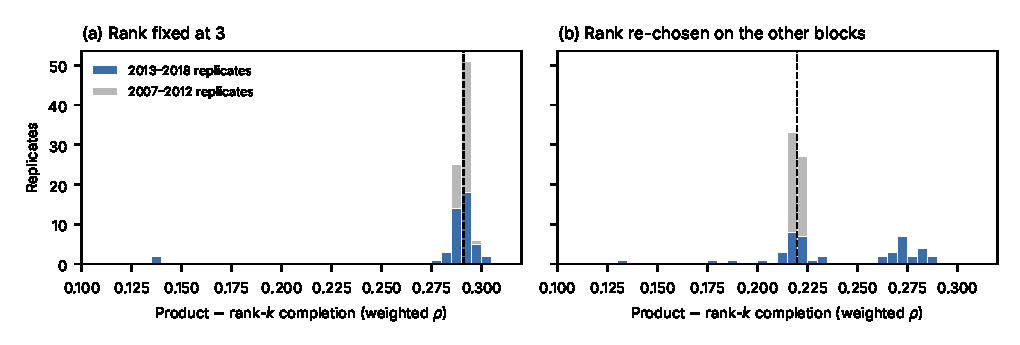
\includegraphics[width=\textwidth]{figS1_block_replicates.pdf}
\caption{Whole relation types withheld: the 90 JRR replicate values of product $-$ rank-$k$ completion (pair-weighted mean of within-block $\rho$), stacked by the period whose replicate it is. (a) Rank fixed at 3, as in Table~S8; (b) rank re-chosen on the other blocks in every replicate. Dashed line: full-sample value. In (a) the two replicates at 0.137 give 98\% of the JRR sum of squares.}
\end{figure*}




























\begin{thebibliography}{S9}
\bibitem[S1]{wright1934} S. Wright, ``The method of path coefficients,'' \emph{Ann. Math. Statist.}, vol.~5, no.~3, pp. 161--215, 1934.
\bibitem[S2]{bollen1989} K. A. Bollen, \emph{Structural Equations With Latent Variables}. New York, NY, USA: Wiley, 1989.
\bibitem[S3]{floyd1962} R. W. Floyd, ``Algorithm 97: Shortest path,'' \emph{Commun. ACM}, vol.~5, no.~6, p.~345, 1962.
\end{thebibliography}
\end{document}
